\documentclass[14pt,a4paper]{extreport}
\usepackage[cp1251]{inputenc}
\usepackage{BSUStyle}
\usepackage{graphicx}
\usepackage{amsmath}
\usepackage{listings}
\usepackage{algorithmic}
\usepackage[ruled,vlined]{algorithm2e}
%\usepackage{refcheck}


\begin{document}

% ****************************************************************************
%   ТИТУЛЬНЫЙ ЛИСТ \\ не трогаем знаки конца строки, название CAPS!
% ***************************************************************************

\title{СИНТЕЗ ОПТИМАЛЬНОЙ СИСТЕМЫ НА ОСНОВЕ МЕТОДОВ ПАРАМЕТРИЧЕСКОГО ЛИНЕЙНОГО ПРОГРАММИРОВАНИЯ}

\author{Селях Никита Евгеньевич}

% \project{Курсовая работа (проект)}
\project{Курсовой проект}

%\spec{прикладная \\ математика}


% для курсовыч
\supervisor{канд. физ.-мат. наук \\ доцент Н.М. Дмитрук}

% для дипломов
% \supervisor{канд. физ.-мат. наук \\ доцент Н.М. Дмитрук}

% для магистерских
%\supervisor{Наталия Михайловна Дмитрук \\ канд. физ.-мат. наук, доцент}

% для курсовых
\BSUtitle

% для дипломов и магистерских
%\BSUtitle

% ************************************************************************
%   ОГЛАВЛЕНИЕ
% ************************************************************************

\addtocontents{toc}{~\hfill{C.}\par}
\tableofcontents

% ************************************************************************
%   ОСНОВНАЯ ЧАСТЬ
% ************************************************************************


\chapter*{��������}
\addcontentsline {toc}{chapter}{��������}


% ������� ���������� ����������� ��� ���� ������������ �����. �� ��������� ��� ����������� ��������� ������� ��� ��� ���� ��������� ��� ��� ������������� ����������� �������� � ��������� ��������������� �������, ��� �������� ��������� �� ��� ��������� �� �������� ����������. ���� �������� � ������� ������� �������� � ����������� �� �������������� �������� � ������ ���, ��� �������, � ������ ��������� �������, �.�. � ����� �� �����, � ����� �������� ��������. � ������� ����������� ������-����������� ��������� ����� �� ���� �������������� ������� ��������� � ������� ����������, ��������������� �� �������� ���������� � �������� �������. ������ �� ����������� ������ ���������� � �������� ������� ������������ ����������� ������� ���������� ������� ����� ������������ ����������.

���������� ��� ������� �� ������ ������������ ����������. �������� ������ �� ���, ���������� ����� �������� �������� ��������� ����������, ������ ������������ ���������� --- ������ ������������ (���������������) ������������� ����������. ������ ������ �������� ������ ������������ ���������� ��� ������ ����������� ������ ����������, �������������� ������������ �������� ������������ ������ ����������. � ������������ � ���� � ������ ������ ��� ������������ ���������� �������� �������������� �����������, �� ������� ������ ��������� ���������� ����������� ��������, � �������� �������� ������ ��������� ������ ������� ������������� ������ (�������������, ��������������, ����������� ����������� �������, ����������� � ����������� ������� ������������� � �.�.).

�� ������ ������ ���������� --- ��� �������, � ������� ��� ���������� ������� ��������� ������� ���������� � ������ ������� ������ ������� ��������� ���������������� (�����������) ����������� �� ������ ���������� � ����������� �� ��������� � ����� ������� ���������� � ��������� ������� � ����������� �� ���� �����������. 

���������� ���������� �����������, ���� (�����������) ����������� ����������� (���������) ����������� �� ��������� ���������� �� ������ �������� ���������� � �� �������������� � �������� ����������. ��� ����������� ���������� (�����������) ����������� ����������� ��������� � �������� ���������� �� ������� ��������, ������� ������������ ����������, ��������� � �������� �������.


���������� ����������� ����������� ����������� ����������� ���������� �������� ����������� ������ ���������� � �������� �������� �������� ������ ������������ ���������� �� ������ ������.

� ������ ��������� ������ ����� ����������� ������������ ������ �������. ��� ���������� ����������� �������� ������ ������ ������������ ���������� ����������� � ��������� �����, ��������� �� ������� �������� ���������� --- ������� ������� � ���������. ���� ������� ������� �� ���������, � ������ ������������� � ������ ���������� ����������, �� ������ ������������ ���������� ����� ��������������� ��� ������ ��������������������� ��������� ����������������.
  
��������������� ���������������� --- ������ ������ ��������������� ����������������, ������������ ��������� ����� �����������, ���������� ���������, � �������� ����� �������� ������� ��� ����� ������������/��������� ������������ ���������� (� ������� �� ������� ����������������, ������� ������� ����� ��������� ����������).

���������� � ��������� ���������������� ���������������� ��������� �������� ��������� �� ���������� � ����� � �������� ������������ �������� ������ ������������� ��������� ������� �� ������ ������� ������ ���������� �� �������������� ������ (Model Predictive Control --- MPC). ��� � ��������� � �������������������� �������� � ������������ ����������������� �������� �������� ������ ���, ��������� ������� ������  --- ��������������� �������� ����� --- ���������� � ����� ����.

� ��������� ������ ����� ����������� �������� ��������� ������ ���, � ����� ���� ���������� �������� ������ �� ������ ���������������� ���������������� ����� ������� �� �������� ������� ����������� �������.

\chapter{����� ����������}\label{chap1}


� ��������� ����� ���������� ����� �������� ����������� ������ ������������ ����������. ������� ����������� ������������ �����, ����������� ��� ����������� ������������ ������ ����������. ����� ���������� �������� ���������� ������������ ������ --- ������� ��������� �.�. ���������� � ������������ ���������������� �. ��������.

� ������ ����� ��������������� �������� ���������� ������ ������������ ����������, ������������ ������ � ����������� �������� ������, � ����� ����������� ���������� � �������� ������� � ���������� ����������� �������� �����

����� ����, ����������� ����������� ������ ���������� � �������� �������: ���������� ����������� �������� ������ � ������� ������������ ���������� � �������� ���������� � ������ ���������� �� �������������� ������ ��� ������� ������������ �������� ������ ����������  --- ������������ ���������� ������������ ������ ��� ������� �����������.

% %%%%%%%%%%%%%%%%%%%%%%%%%%%%%%%%%%%%%%%%%%%%%%%%%%%%%%%%%%%%%%%%%%%%%%%%%%%%%%%%
% \section{������ ���������� ������}\label{1sec:snth}
% %%%%%%%%%%%%%%%%%%%%%%%%%%%%%%%%%%%%%%%%%%%%%%%%%%%%%%%%%%%%%%%%%%%%%%%%%%%%%%%%


% ������ �� �������� � ������ ������������ ����������, ������� �������� � �������� ���������� ����� ���������, ����������� �������� ������� � ��������� ����������������, ��� �������� ���������� ������������ ������������ ����������� ���������� ��������. ����� �������, ����� �������������� �������� ������ ������� �������������� ��������� �� (��������� ������) � ������� ��������������� ����������.
% ��������� ������ ������� � ������ ��������� � ��������� ����������, ��������������� ������� �������� �������. ��� ���� ������ �������������� ����������� ������� �� ���������� ������ ��� ���������� ���������. ������ ����������� �� ������ ����� ���������� �������� � ���������� ����������� ���������, ���������� ������� ���������� ��������� � ����������, � ����� ��������� ����������� ���������. ���������� �� ���� ����� ������ ��� ����� �� �������� ������������ ��������. ���� ���� �������������� �� ����� ���� ������� �������������� ������ � ��������� � ������� ����������� ���������.
% �������������� ������ ������������� �������� ����� ���������� ���������, ������� ������� �������� ������ ������������ ������� � ��� ���� �� ������� �������������� ����������������� ����������. �� ������ ����������� ������ ���������� ��������, ��� ��������� ����� ���� ����������������, ������������, ��������� �� ���� �������� �������� ����� � ���������. � �������������� ������� ��� ��� ������������, ��� ��� ��������������� ������� ������ ���� ����� ���� ����������� �������������� ������ ������� ����.
% ��������� ������ �������������� �� �������� ���������� �������� ������� ���������� ������������ ���������. ��� ������� ���� ������ ���������� ��� �������: 1) ����������������, ������� �������� � ������ ������������ ���������� ��� ���������� ������� � ���������� �������������; 2) ������������� ������� ���� ���������� ���������� ������ ������������ ������� � ����������� ������ ���������� �������� ������ ���������� ������; 3) ������ ������ ��������� ���������� ��� ������������ ������� ��� �����-���� ��������� � �������������.
% ������ ��� ������� �������� ������������ � ���������� ������������ ������ ����� ������ ������ � ����� ��������� ��������� ���������� ������ ������������ (����������� ��� ����������) ������.   � ������ ������� ������������ ������� �������� ����� (����������� ��������, ����������� ���������� � ��������������) � ������� ����������� �������������� ������� � ������������ ������ ������� ����������� ������. ��� ���� ������ ������������� ����������� ����������� ���������� �� ��������� �������� ��������� �������. ��� �������������

% ������� ������� �� ����������� ��������� ������� � ����������� ����� ��������� �����������, ��� ����� �������� � ��������� ������� ��������� � �������������� �������� ���������� ������� �������� ���������. ������ ���������� ������ ������������� ������� ������� � ���, ��� ���������� � �������, ���������������� � ����������� �������, �� ������ ����� ��������� � ��������������� ������������������ ���������� ��������. �� ����������� ����� � ������ ���������� ������ ���������� �������� �������� ��������� ������ ������� ������� � �������. �� ������ ��� ������� � ���, ��� ����������� ������ �������������� ����� ��������� � ����������������� ��������.
% ������������� � ������ ���� �������� ����������� ����������� ������ �������, ������� ��������� �������� ��������� ��� ���������� ����������. � ���� ������� ��������� [13]:
% 	�	������������������ ������ ����������� ������������� ������� ���: ��������, ��������� ���������, ����������� ���������� �������������, ���������;
% 	�	������������� ������ ������������ � ����������� ����������;
% 	�	������ ��� �� ������������ ��������� �������� (������������) �������� ������������� ����������, ������������� ��������� � ����������� ��������������� ����������������, ��������� ��������� ����������, ������� ������-�����, �������� ���������� ����������, �������� �������������� ��������������� ����������� ����������� � ��.
% ��� �������� ������� ����������� ��� � �������������� ������������������� ������������ ����������� �� ������ ������� ����������� � ��������� ������������� ���. �� ��������� � ������� ����� �������� ����� ����������� �������� ������ ������������ ������� � ������ ��� � ������  ����  ������������  �������  ����������.  ������������� � ������������������ ������, � ���� �������, ��������� ����������� ��� � ����� ����� ���� � ����� ����������� ������� ����� ��������� �������.

%%%%%%%%%%%%%%%%%%%%%%%%%%%%%%%%%%%%%%%%%%%%%%%%%%%%%%%%%%%%%%%%%%%%%%%%%%%%%%%%
\section{�������� ���������� ������ ������������ ����������}\label{1sec:optimal-control}
%%%%%%%%%%%%%%%%%%%%%%%%%%%%%%%%%%%%%%%%%%%%%%%%%%%%%%%%%%%%%%%%%%%%%%%%%%%%%%%%

���������� ����� ���������� ������ ������������ ���������� �������� � ���� 5 ����������� ���������: ���������� ����������, �������������� ������ ������������ �������, ����� ���������� � ����������� �� ���, ����������� �� ������� ����������,
�������� ��������.
���������� �� ���������.

1) ���������� ����������. ������ ����� ������ ������������ ���������� ����������� �� �����������, ��������������� �� ��������� ���������� ������� $T = [t_{0},t_{f}]$, � ����������, � ������� ������������ ������� ��������������� � ���������� ������� ������� $k = 0,1,...N$, ��� $N$ � ����������� �����.

�� ����������������� �������� ����������� ������ � ������������� � ��������������� �������� ��������� ��������. ���������� ����� ������ �� ����������� ���������.

2) �������������� ������. �������� ���������� �������� ������������, ��� �������, ����������������� (��� ����������� ������)

\begin{equation}\label{1v}
\dot{x}(t) = f(x(t),u(t),t), t \in [t_0,t_f],
\end{equation}
��� ����������� ����������� (��� ���������� ������)

$$x(k + 1) = f(x(k),u(k),k),k = 0,1,...,$$
��� $n$-������ $x$ ���������� ���������� �������, $r$-������ $u$ ����������
�����������, ������� 
$ f : R \times\ R^r \times R \rightarrow R^n$ ������.

����� ���������� ��������� $n$ ���������� �������� ������� ����������, ����� $r$ � ������ ������.

����� ����� ������������� ����������� ������� ���� (\ref{1v}).

3) ����� ���������� � ����������� �� ���. ��� ������������ �������� ���������� ����������� ����� �������, �� �������� ���������� ����������. ��� ����� ����: ���������, ����������, �������-�����������, �������, ���������� ������� � �.�.

����� ������ ��������� ���������� �������� ��������� 
$U \subset\ R$ � ��������� ���������� �������� ����������. ��� �������, $U$ � ������� � $R^r$.

����� ����� ������������� ���������� �� ������ �������-����������� �������.

\begin{definition}�������-����������� ������� $u(\cdot) = (u(t),t \in [t_{0},t_{f}])$ ���������� ��������� �����������, ���� $u(t) \in U, t \in [t_{0},t_{f}].$
\end{definition}

4) ����������� �� ������� ����������. ����������� �� ���������� ��������� ����� �������������:\begin{itemize}
\item � ��������� ������ ������� $t_{0}$:
$$x(t_{0}) \in X_{0};$$
\item � �������� ������ ������� $t_{f}$ --- ����� ����������� ���������� �������������: $$x(t_{f}) \in X_{f};$$
\item � ������������� ������� $t_{i} \in [t_{0},t_{f}], i = \overline{1,m},$ �� ���������� ���������� � ������������� ������� �����������:
$$X(t_{i}) \in X_{i},i = \overline{1,m},$$
\item �� ���� ���������� ���������� � ������� �����������:
$$x(t) \in X(t),t \in [t_{0},t_{f}],$$ ��� $X_{0}, X_{f}, X_{i}, i = \overline{1,m}, X(t), t \in [t_0,t_f],$ � �������� ������������ ������������ ���������.
\end{itemize}
 ������ ���������� � $x(t_f) \in X_f $ ����������:\begin{itemize}
  \item ������� �� ��������� ������ ������ ����������, ����
 $X_f = R^n$, \item ������� � ������������ ������ ������ ����������, ���� $X_{f} = \{x_{f}\}$, \item ������� � ��������� ������ ������ ����������, ���� $X_{f}$ �������� ����� ����� ����� � �� ��������� � $R^{n}$.
\end{itemize}
 ����������� ������������� ����� ����� ��� ����� � ������������� �� ����� ����� ���������� $x_{0} \in X_{0}$.

  �������� ����� ��������� �����������, ����������� ����� ����� ����������� ��������� � ����������� ����������:
$$(u(t),x(t)) \in S \subseteq R^r \times R^n,t \in [t_{0},t_{f}[.$$ \begin{definition} ��������� ���������� $u(\cdot)$ ���������� ���������� (���, ����������), ���� ��� ��������� ���������� $x(\cdot)=(x(t), t \in [t_0,t_f]$, ��������������� ���� �������� ������������ ������. \end{definition}

5) �������� ��������. �������� ����������� ���������� ����������� ��� ���������� ��������� ��������

 ���������� ������ ���� �������� ��������:

i) �������� �������� ������ (������������ ��������)
$$J(u) = \varphi(x(t_{f})),$$

ii) �������� �������� �������� (������������ ��������)
$$J(u) =\int^{t_{f}}_{ t_{0}}
f_{0}(x(t),u(t),t)dt,$$

iii) �������� �������� ������
$$J(u) = \varphi(x(t_{f})) +
\int^{t_{f}}_{ t_{0}}
f_0(x(t),u(t),t)dt,$$

iv) ������ �������������� (�������� �������� � ��������������� ������������������ ��������).
$$J(u) = t_{f} - t_{0} \rightarrow \min.$$
\begin{definition} ���������� ���������� $u^{0}(\cdot)$ ���������� ����������� ����������� (����������� ����������), ���� �� ��� �������� �������� ��������� �������������� �������� (min ��� max):
$$J(u^0) = extr J(u),$$

��� ������� (��������) ������� �� ���� ���������� �����������.
\end{definition}
%%%%%%%%%%%%%%%%%%%%%%%%%%%%%%%%%%%%%%%%%%%%%%%%%%%%%%%%%%%%%%%%%%%%%%%%%%%%%%%%
\section{������� ��������� � ������������ ����������������}\label{1sec:pm} % xxx �������� �� ���� �����
%%%%%%%%%%%%%%%%%%%%%%%%%%%%%%%%%%%%%%%%%%%%%%%%%%%%%%%%%%%%%%%%%%%%%%%%%%%%%%%%
� ������ ������������ ���������� ���������� ��� ��������������� ����������: ������� ��������� �.�. ����������\cite{Pontryagin} � ������������ ���������������� �. ��������.\cite{Bellman} �������� ��� ���������� �� ������� ���������� ������ ������������ ����������.

 $$J(u) = \varphi(x(t_{f})) +
\int^{t_{f}}_{ t_{0}}
f_0(x(t),u(t),t)dt \rightarrow \min, $$
 \begin{equation}\label{tr2}\dot{x}(t)=f(x(t),u(t),t), x(t_0)=x_0,\end{equation}
$$u(t) \in U, t\in [t_0,t_f].$$

\subsection{������� ��������� ����������}

��������� ��������� ���������� �������� ����������� ������� ������������� � ������� ������������ ����������, ��������� � ������������� �������������:

$$H(x,\psi, u, t) = \psi 'f(x, u, t) - f_0(x, u, t) = \sum^n_{j=1} \psi_j f_j(x, u, t) - f_0(x, u, t).$$ ����� $\psi = \psi (t) \in R^n $ --- ����������� ����������.
\begin{theorem}����� $u^0(\cdot), x^0(\cdot)$ � ����������� ���������� � ���������� � ������ (\ref{tr2}), $\psi^0(\cdot)$ � ��������������� ������� ����������� �������
$$ \dot{\psi}^0(t)= -\frac{\partial H}{\partial x}(x^0(t),\psi^0(t),u^0(t),t),$$ � ��������� ��������
$$\psi^0(t_f) = - \frac{\partial\varphi}{\partial x}(x^0(t_f)). $$
����� ��� ������ $t \in [t_0,t_f]$, ���������� $u^0(t)$ ������������� �������:
$$H(x^0(t),\psi^0(t),u^0(t),t) = \max_{v\in U}
H(x^0(t),\psi^0(t),v,t), t \in [t_0,t_f].$$
\end{theorem}

��� ���� ����� ������ ������ � ������� �������� ��������� ������ ��������� ��������� �������. ������� $H(x, \psi ,u,t)$ ������������� ��� ������� $r$  ���������� $u = (u_1,...,u_r).$ ����� �������� ���������� ����������� ��� ������� �������������� ������ $(x, \psi ,t)$
\begin{equation}\label{krz}u(x, \psi ,t) = \arg \max_{v \in U} H(x, \psi , v, t).\end{equation}
���� �������� ������ (\ref{tr2}) ����� �������, ������� (\ref{krz}) ���������� �� �������� ��������� �������� $(x, \psi , t).$

�����  $u$ � ���� (\ref{krz}) �������, ����� ����� ����������� ��������� ������� � ���������� ���������:
$$ \dot{x} =\frac{\partial{H}}{\partial{\psi}}(x, \psi , u(x, \psi , t), t) = f(x, \psi , u(x, \psi , t), t), \ x(t_0) = x_0,$$
$$ \dot{\psi } = - \frac{\partial{H}}{\partial{x}}(x, \psi , u(x, \psi , t), t), \  \psi (t_f) = -\frac{\partial{\varphi(x(t_f))}}{\partial{x}}.$$
����� ������� �������� ����������� ������� ������, ������� ���������� ������� ������� �������� ���������.

����� �������, ��� ������� ���� ��������� ������������� ���� ������� $x(\cdot), \psi (\cdot),$ ��������������� ������� ������ �������� ���������. ��������� ���� ����� ���� � (\ref{krz}), �������:
\begin{equation}\label{prtn}u(t) = u(x(t), \psi (t),t), t \in [t_0, t_f],\end{equation}
������� ������������� �������� ��������� �, ������, ����� ������������ �� ���� ������������ ����������, � ������� $x(t) = x(t\mid t_0,x_0,u(\cdot)), t\in [t_0, t_f],$ --- �� ���� ����������� ���������� � ������.

�������, ��� ������� ��������� � ������ (\ref{tr2}) �������� ���� ����������� �������� �������������, ������� ����������� ���������� �� ����� ���� �����������. ����������� ������� ���������� ����������� ���������� (\ref{prtn}).
\subsection{������������ ����������������}

���������� ������ (\ref{tr2}) � �����������, ��� ��� ����� �������. ������ ������������� ����������������\cite{Bellman}, �������� ������ (\ref{tr2}) � ��������� �����
$$ J_{\tau ,z}(u) = \varphi (x(t_f)) + \int^{t_{f}}_{\tau }
f_0(x(t),u(t),t)dt \rightarrow \min, $$
 \begin{equation}\label{dp1}\dot{x}(t)=f(x,u), \  x(\tau )=z,\end{equation}
$$u(t) \in U, \ t\in T = [\tau ,t_f],$$
��������� �� ������� $\tau \in T$ � $n$-������� $z.$

���� $(\tau , z)$ ������� �������� � ������ (\ref{tr2}). ��������� ����� $$B(\tau ,z) = \min J_{\tau ,z} (u)$$
����������� �������� �������� �������� � ������ (\ref{dp1}) ��� ������� $(\tau , z)$. ���� ��� �������  $(\tau , z)$ ������ (\ref{dp1}) �� ����� �������, ������� $B(\tau ,z) =  +\infty$. ����� $$X_{\tau } = \{z \in R : B(\tau ,z) < +\infty \}.$$
�������\begin{equation}\label{fb} B(\tau ,z), z \in X_{\tau}, \tau \in T,\end{equation} �������� �������� ��������.

��������� � ������� �����������, �������� ������������� ������� (\ref{fb}), �������� ���������� ��������
\begin{equation}\label{ub} -\frac{\partial B(\tau,z)}{\partial\tau} = \min_{v \in U}\left\{ \frac{\partial B'(\tau,z)}{\partial z}f(z,v) + f_0(z,v)\right\}, z \in X_\tau, \tau \in T.\end{equation}
������� �� ��������� (\ref{dp1}) ������ � $\tau = t_f$, ������� ��������� ������� ��� ��������� ��������
\begin{equation}\label{gusl}B(t_f,z)=\begin{cases}
\varphi(z), ���� z \in X, \\
+\infty , z \not\in X.
\end{cases}\end{equation}
\bigskip

����� ���������� ������������� ���������������� ������� � ���������: ��� ����� ������������ ��������� ��������. �� ������� ��������� ��������� ����������� �������.

%%%%%%%%%%%%%%%%%%%%%%%%%%%%%%%%%%%%%%%%%%%%%%%%%%%%%%%%%%%%%%%%%%%%%%%%%%%%%%%%
\section{������������ ������ � ���������� ����������� �������� ������}\label{1sec:MPC}
%%%%%%%%%%%%%%%%%%%%%%%%%%%%%%%%%%%%%%%%%%%%%%%%%%%%%%%%%%%%%%%%%%%%%%%%%%%%%%%%

��������������� ������ ������������ ���������� ������������� ��������� � �������� ����������������. � ������� �� ������������� �������, � ������� ����������� �������� ����� �������� �� ����������������� �������, � ������ ������������ �������������� ������ � ������������� �����������������. ���������� � ����������� ���������� ����������� ������������ ��������� \\

\begin{equation} \label{1problem}
    J(u) = \varphi(x(t_f))\to \min,
    \end{equation}
\begin{equation} \label{2problem}
    \dot{x}=f(x,u,t),\ x(t_0)=x_0
     \end{equation}
\begin{equation} \label{3problem}
  	x(t)\in X\in\mathbb{R}^n
     \end{equation}
\begin{equation} \label{4problem}
  	 u(t)\in U\in\mathbb{R}^r,\  t\in [t_0, t_f]
     \end{equation} 


� ������������ ������ ����� ��������������� �������� �������� (\ref{1problem}) �� ����������� ������� (\ref{2problem}), ������� � ������ ������ ������� ����� � �������� ��������� X (\ref{3problem}) � ������� ������������ ����������� ����������� (\ref{4problem}).
(\ref{1problem}) - (\ref{4problem}):  $t_0, t_f$ --- ������,\\
$x = x(t)\in\mathbb{R}^n$ --- ��������� ������� ���������� � t,\\
$u = u(t)\in\mathbb{R}^r$ --- �������� ������������ ����������� � t.\\
$f:\mathbb{R}^n\times\mathbb{R}^r\times\mathbb{R}^n$ ������������ ������������� � ������������� ������� ��������� (\ref{2problem}) �� ���������� ������� $T = [t_0; t_f]$. \\

������ (\ref{1problem}) - (\ref{4problem}) ����� ������������� � ������ �������-����������� ����������� ����������� u.
���������� ����������� ���������� (���������) --- �������-����������� ������� $u(\cdot)\in U$,
���� ��� ��������� ���������� � ������� (\ref{2problem}), ��������������� (\ref{3problem}). ���������� ����������� ���������� - ����������� (����������� ���������), ���� �� ��� �������� �������� (\ref{1problem}) ��������� ������������ ��������.
$J(u^0) = min J(u)$, ��� ������� ������� �� ���� ����������.\\
��� �������� ������� ������������ ����������� �������� ����� �������� ������ (\ref{1problem}) - (\ref{4problem}) � ��������� ��������� �����:

\begin{equation} \label{5problem}
    \varphi(x(t_f))\to \min,
    \dot{x}=f(x,u,t),\ x(z)=z
  	x(t)\in X\\
  	 u(t)\in U,\  t\in [\tau, t_f]
     \end{equation}

����� $u^0(t|\tau,z),\ t\in T_\tau$ --- ����������� ��������� ������ (\ref{5problem}) ��� ������� $(\tau,z)$ \\
$X_\tau$ --- ��������� ��������� z �����, ��� ��� ������� $(\tau,z)$ ���������� ����������� ������� ������ (\ref{5problem}) \\
�������
\begin{equation} \label{6problem}
    u^0(\tau,z) = u^0(t|\tau,z)
     \end{equation}
     --- ����������� �������� �����.\\

���������� (\ref{6problem}) --- ������ ����������� ������� ����������.\\
����������� ������� (\ref{6problem}) � ��������� (\ref{3problem}) --- ��������� ������� ����������
\begin{equation} \label{7problem}
    \dot{x}=f(x,u^0(t,x),t),\ x(t_0)=x_0
     \end{equation}
���������� ��������� --- �������������� ������ ����������� �������������� ������� ����������.\\
��� ������ ��������� $x_0$ ������� ��������� (\ref{7problem}) � ��������� ���������� $x(t_0)=x_0$ --- ����������� ���������� ��� ������ (\ref{1problem}) - (\ref{4problem}).\\
�������, ��� ���� ����������� �������� ����� ��������� � ������ �������-����������� ����������, �� �� ������ ������� ��������� (\ref{7problem}) ������������ �����
���������������� ��������� � ��������� ������ ������ �, ������ ������, �� ����� ������������� �������. � ���� ������� ���������� ���������� �������.

����� �������� ������������� ����������, ����� ��� ����������� ������� ��������� ������� ����������, � ������ ������������ ���������� (\ref{1problem}) - (\ref{4problem})
�������� �� ������ �������-����������� ��������� ���������� � ���������� �����������.\\
�������� � �� $n\in N$ ������ $h = \frac{t_f - t_0}{N}$

\begin{equation}
    u(t) = u(s),\ t\in [s, s+h],\ s\in T_h = \{t_0, t_0 + h, ..., t_f - h\}
     \end{equation}
������� ��������� � ����������� ��������� � ������ ���������� ���������� ���������� ����������� � ������ �������-����������� ����������.\\
���������, � ������� ������������ ������ (\ref{1problem}) - (\ref{4problem}) ����� ��������� ��������� �������:
\begin{equation} \label{8problem}
    \varphi(x(t_f))\to \min,
    \dot{x}=f(x,u,t),\ x(z)=z,\ 
  	 u(t)\in U,\  t\in T_h.
     \end{equation}

��������� ������� �� $(\tau,z), z\in \mathbb{X},\ \tau\in T_h$,\\
����������� ���������� �������� ����� --- ������� 
\begin{equation} \label{9problem}
    u^0(\tau,z) = u^0(t|\tau,z),\  z \in X_\tau,\ \tau \in T_h,
\end{equation}

\section{����������� ���������� � �������� ������� � ���������� ����������� �������� �����}\label{1sec:real-time}
��������������, ��� ������������ $u^0(\tau,z) = u^0(t|\tau,z),\ \tau\in T_h,\ z\in \mathbb{X_\tau}$.\\
��������� ������� ����� ������� ������� ����������� ����������� $u^*(t), t\in T$ � ���������� $x^*(t), t\in T$ ��������������� ���������
$x^*(t) \equiv f(x^*(t), u^*(t), t) + w^*(t), t\in T, x^*(t_0) = x_0$
\begin{equation} \label{9problem}
    u^*(t), t\in T: u^*(t) = u^0(\tau,x^*(z)), t\in [\tau, \tau + h], \tau\in T_h.
     \end{equation}
--- ���������� ����������� �������� ����� (\ref{1problem}) � ���������� �������� ����������.\\
������ �����, ��� � ���������� �������� ���������� ����������� �������� ����� (\ref{1problem}) �� ������������ ������� �� ���� ������� �� �����������.
����� ���� �� �������� ����� ����� ������������������ ���������� ��������� ����������� ������� $x^*(\tau), \tau\in T_h$, � ���������� �����
��� ������ ������� ������� $(\tau,x^*(\tau)), \tau\in T_h$, ��������� �������� ���������� 
$u^*(t) = u^0(\tau, x^*(\tau)),\ t\in [\tau, \tau + h]$ ����������� �������� ����� �� ����� $s(\tau)<h$\\
����� ��������, ��� ������� ���������� �������������� � �������� �������, ���� ��� ������� �������� ������� $\tau\in T_h$ ������� $u^*(\tau)$
����������� �� ����� $s(\tau)<h$, �.�. �� ��������� ���������� ��������� $x^*(\tau+h)$. ����������, ��������� ����������� ����������� �������� ����� � �������� �������
����� �������� ����������� �����������.\\
����� �������, � �������������� �������� ���������� � �������� ������� ������ ������� �� ���� �� �������� � ���������� ��������� ������ ������������ ����������.


%%%%%%%%%%%%%%%%%%%%%%%%%%%%%%%%%%%%%%%%%%%%%%%%%%%%%%%%%%%%%%%%%%%%%%%%%%%%%%%%
\section{������ ���������� �� �������������� ������ MPC}\label{2sec:mpc-general}
%%%%%%%%%%%%%%%%%%%%%%%%%%%%%%%%%%%%%%%%%%%%%%%%%%%%%%%%%%%%%%%%%%%%%%%%%%%%%%%%

���������� ������
$$
\begin{cases}
    \dot{x} = f(x, u),\ u(t) \in U, \\
    x(0) = x_0 ,\ x(\tau) \in X.
\end{cases}
$$
$$\min_{u} J = \int_{t}^{\inf} F(x(\tau), u(\tau)) d\tau$$


$\varphi(t)$ --- ���������, ���� $\forall \varepsilon > 0 \ \exists \delta(\varepsilon) > 0 \ \| x(0) - \varphi(0)\| \le \delta \Rightarrow \| x(t) - \varphi(t) \| \le \varepsilon$\\

���������������� ������������:
\begin{enumerate}
    \item $\varphi (t)$ --- ���������
    \item $\exists \delta \ \| x(0) - \varphi(0)\| \le \delta \ \lim \lim_{t\to\infty} \| x(t) - \varphi(t) \| = 0$\\
\end{enumerate}
��������: 
$$
\begin{cases}
    \dot{x} = f(x, u),\ x \in \mathbb{R}^n, \\
    x(0) = x_0 ,\ u \in  \mathbb{R}^m.
\end{cases}
$$ \\
�����������: \\
$$x(t) \in X,\ u(t) \in U \ \forall t \ge 0.$$\\
������ MPC:
� ������ ������� $t$, ���� ��������� ��������� $x(t)$

$$ \min_{\overline{u}(:,t)} J(x(t), \overline{u}(\cdot,t)) $$ \\
$\overline{u}$ --- ������������� \\
$u(t, \tau)$ --- $u(t)$ � ������������� ������ ������� $\tau$
$$ J(x(t), \overline{u}(\cdot,t)) = \int_{t}^{t + T} L(\overline{x}(\tau, t), \overline{u}(\tau, t)) d\tau,$$ \\
$$\dot{\overline{x}} = f(\overline{x}, \overline{u}), \\$$
$$\overline{x}(t,t) = x(t), \\$$
$$\overline{u}(\tau, t) \in U, \\$$
$$\overline{x}(\tau, t) \in X, \ \forall \tau \in [t, t + T]. $$

$L$ --- ��������� �����,\ $\delta$ --- ��� �������������.

\chapter{��������������� �������� ����������������}\label{chap2}

������ ��������������� ����������������, ����� ��� ��������, ��������, ���������� ����������������, ������ ���������� ����������� �������� ������������ --- ��������� --- ��������, ��������, ������� ������� ��� �������������� �����������. ��������� ������� \textit{����� ����������} ���� ���������� �� ������� ������ (����������� ����, ����������� �������� ������� �������) �������� ������ ����������������. � ������ �������, ���������� ��� ���������� �����, � ������� ������� ������������ �������������� ������� ��� ������� ��������� �������� ����������. ������ ������ ��������������� ����������������, ������������ ������������� ����� ����� ���������� \textit{��������������� ����������������}. ��� ���� ������ ��������������� ���������������� ��������� � �������, � ������� ����������� ������� ���������� ���������, � �� ����� ��� ��������� ����� � ���������� ����������� ���������� �������������������� ����������������.

��� ���������� �� ��������, �������������������� ���������������� --- �������� ���������� ���������� ����������� � ��������������� �������� ������ � ������ ��������� ������. � ����� � ����, � ��������� ����� ���������� �������� �����������, ������� � ��������� ���������� ������� � ������� ��������������������� ����������������.

%���� ��������� ������ ��� ������ ����������� ������� �������������������� ��������. ��� �������, �������������� ��������� ���������� ���������������� ��-�� ��������, ������� ���� ����������, ���� ����� ������ �����. ��������������� ���������������� �������������� ������������ ������������ ���������� �� ����������� �������, ������� ���������� ������������ � ��������������� �������������� � ����������� �� �������������� ����������, �, �������������, ������������� ����, ������������ �������, ������ ����� ��������� �����������.


%%%%%%%%%%%%%%%%%%%%%%%%%%%%%%%%%%%%%%%%%%%%%%%%%%%%%%%%%%%%%%%%%%%%%%%%%%%%%%%%
\section{����� ���������}\label{2sec:gabella}
%%%%%%%%%%%%%%%%%%%%%%%%%%%%%%%%%%%%%%%%%%%%%%%%%%%%%%%%%%%%%%%%%%%%%%%%%%%%%%%%

������ ����� ������� ��������������� ����� ��������� ���������������� ��� ��������� � ������ \cite{GassSaaty} � 1955 �., � ����� ������ � ������� \cite{GalNedoma} � \cite{Bemporad}. ������� � ��������������������� ���������������� ������ � ��������� ������ ������ � ������������ ����������. ��� ������� � ���, ��� ��� ������������ ������ � ���������� �������� ������ ������������ ���������� � ������������� �� ���������� � ��������� � �������� ���������� ���������� ����� ���� �������������� ��� ������ ��������������� ����������������. ��� ����� ������ ��������� ��� ��������� ���������������� ��� �������� ������ � ��������� ��� ��������� ������������� � ������������� ��� ������ ����������� ����������������. ��� ����������� � ����� 1, ������� � ����� ������� ������������ ���������� ����������� �������� �����, ��� ������� ������� --- ����, � ����� ������, ��������� �� ������� ������� � ��������� ������� � ���� ������. ����� ����������, �� �������� ������� �������� �������� � �����������, �������� ������� ������������� ��������.

��������� �������������������� ����������������, ����� ���������������� � ��������� ������� ������ ������������ ���������� � ����� ���� ��� ������� ������� �� ��������� ������������� ��������� ���������� �������.

� ������ ���������� �� �������������� ������, ��� ����������� � ����. \ref{}, ���������, ����� �������������� ������ ������������ ���������� ��������  � �������� ������� ��� ���������� �������� ������������ �����������. �������������� ������ ������� �� �������� ��������� ������� ����������, ������� ������� � �������� ���������� ��������� � �������������� ������ � ��������� � �������� ���������. � ������� ��������������������� ���������������� ������� � �������� ������� (������) ����� ���� ���������� �������, �� ������ �������� ����������. ����� � �������� ������� ��� ���������� �������� � ���������� ������� ������ ��������������������� ���������������� ��� ����������� �������� ���������, ��� ����������� ����� ������� �������������� ������ ������������ ����������.



�������������������� ������ ���������� ������� ����������� ������� --- ������������ ���������� ������ ���������������� ����������������, � ������� ��������� ������� ������������� �������� �����������. � ���� ����� ������� �������� �������� ���������� ����������� ��������������������� ���������������� �� ������ \cite{Gal}, � ���������, ����������, ���������� ����������� ����������� ������� �� ����������, ����������� ��������������� �����, ������� ����������� �������. ����� ������ ��������� ������� �������������������� ����� ��������� ���������������� (mp-LP) � �������������������� ����� ������������� ���������������� (mp-QP). 

�������� ���� ����������, �������������� � ���� �����, ������� � ���, ����� ��������� ����������� ������� � ����������� ��������� �������� ���������, ��������� ����������� � ����������� ������� �������������, � ����� ���������� ��������� ������������ ���������� �� ������� ���� �������. ��� ��������� ����������� ������ � ����������, ���� �������� ����������� ���������� ��������� ������� ������� ����� ����������� ����������������.


%%%%%%%%%%%%%%%%%%%%%%%%%%%%%%%%%%%%%%%%%%%%%%%%%%%%%%%%%%%%%%%%%%%%%%%%%%%%%%%%
\section{����������� ����������� ������� �� ���������� � ����� �������������������� �������}\label{2sec:results-multy-parametric}
%%%%%%%%%%%%%%%%%%%%%%%%%%%%%%%%%%%%%%%%%%%%%%%%%%%%%%%%%%%%%%%%%%%%%%%%%%%%%%%%

���������� ������ ����������� ����������������, ��������� �� ��������� $x$, ������� ������ � ������� ������� � � �����������:
\begin{align} \label{1function}
   & J^0(x) =  \min_{z} f(z,x),\\
   & g(z,x)\le 0,\nonumber
\end{align}
��� $z \in M \subseteq \mathbb{R}^s$ --- ���������� �����������, $x \in X \subseteq \mathbb{R}^n$ --- ��������,\ $f: \mathbb{R}^s\times\mathbb{R}^n \to \mathbb{R}$ --- ������� �������, � ������� $g: \mathbb{R}^s\times\mathbb{R}^n \to R^{n_g}$ ������ �����������, $g_{i}(z, x)$ --- $i$-�� ���������� ������-������� $g(x, z)$.



����� �������� ��������� $x$ � ������ ��������������� ���������������� (\ref{1function}) � ����������� �� ������� ������� $f$ � $g$ ����� ��������� � ����� ��������� ������������ ������� ��� ������� ��������� $x$, �� ����� � ������ ��� ������������ ��������. ���� ������������ ��������� --- ���������� ��� ��������.

��� �������� �������� ��������� $x$ ���������:
\begin{itemize}
\item $R(x)$ --- ���������� ��������� ���������� $z$ (��������� ������) ������ (\ref{1function}) ��� ������������� �������� ���������:
\begin{equation} \label{2function}
    R(x) = \{z \in M \ |\  g(z,x) \le 0 \};
\end{equation}
\item  $K^*$ --- ��������� ���������� �������� ���������, �. �.
\begin{equation} \label{3function}
    K^* = \{x \in \mathbb{R}^n \ |\  R(x) \not= \varnothing \};
\end{equation}

\item $J^0(x)$ --- ����������� �������� ������ (\ref{1function}): 
\begin{equation} \label{4function}
    J^0(x) = \inf_{z}\{f(z,x) \ | \ z \in R(x) \};
\end{equation}

\item $Z^0(x)$ --- ��������� ����������� ������� (����������� ������) ������ (\ref{1function}):
\begin{equation} \label{5function}
    Z^0(x) = \{ z \in R(x) \ | \ f(z,x) = J^0(x) \}.
\end{equation}
\end{itemize}

��������� $Z^0(x)$ ��� ��������� ����� �������� ����������� ����������. ���� $Z^0(x)$ �������� ������������ ���������� ��� ���� $x$ (������ ����� ������������ �������), �� $z^0(x) \triangleq Z^0(x)$ ����� �������� ����������� ������. 

����� ������������, ��� $K^*$ �������� � $J^0(x)$ ������� ��� ���� $x\in K^*$.

��� ����, ����� ������� $J^0(x)$ � ����������� ��������� $Z^0(x)$ �������� �������� ����������, ������ ����� ������� ������������� ����������� $R: x\mapsto R(x) \subseteq M$. ����� ��� �����������.

%�����������
\begin{definition}
    �����������  $R(x)$ ������� � ����� $\overline{x} \in K^*$, ���� ��� ������������������ $\{ x^{k}\} \subset K^*,\ x^{k} \to \overline{x} $ � ����� $\overline{z} \in R(\overline{x})$ ���������� ����� ����� $m$ � ������������������ $\{ z^{k} \in M \}$ �����, ��� $z^{k} \in R(x^{k})$ ��� $k \geq m$ � $z^{k} \to \overline{z}$.
\end{definition}


\begin{definition}
    ����������� $R(x)$ �������� � ����� $\overline{x} \in K^*$, ���� $\{ x^{k}\}\subset K^*,\ x^{k} \to \overline{x},\ z^{k} \in R(x^{k}) $, � $z^{k} \to \overline{z}$ ������  $\overline{z} \in R(\overline{x})$.
\end{definition}


\begin{definition}
    ����������� $R(x)$ ���������� � ����� $\overline{x} \in K^*$, ���� ��� ������� � �������� � ����� $\overline{x}$. $R$ ���������� � $K^*$, ���� $R$ ���������� ��� ������ $x\in K^*$.
\end{definition}

�� ������ ����������� ����������� �������� ������������� ����������� �������������� ��������������. ������ ����������  ����������� ������� ������������� ����������� $R$ �� ������ ������� �������, �������� ����������� ������ (\ref{1function}).

%�������
\begin{theorem}\label{1theorem}\cite{}
     ����� ����������� ��������� �������: 1) $M$ �������; 2) ��� ������� $g_{i} (z, x)$ ���������� �� $M \times X$ � ������� �� $z$ ��� ������� �������������� $x \in X$; 3) ���������� ����� $\overline{z}$, ��� $g(\overline{z}, \overline{x}) < 0$. ����� $R (x)$ --- ����������� �����������.
\end{theorem}


\begin{theorem}\label{2theorem}\cite{}
    ����� ����������� ��������� �������: 1) $M$ �������; 2) ��� ������� $g_{i} (z, x)$ ���������� �� $M \times X$ � ������� �� $z$ � $x$. ����� $R (x)$ --- ����������� �����������.
\end{theorem}

��������� ��� ������� ���� ����������� ������� ������������� ������������ ��������  �������� � ������������ ����� � ������ (\ref{1function}).

\begin{theorem}\label{3theorem}
    ���������� ������ (\ref{1function}). ���� $R (x)$ --- ����������� ����������� � ������� $f (z, x)$ ����������, �� $J^0(x)$, $x\in K^*$ ����������.
\end{theorem}


\begin{theorem}\label{4theorem}
    ���������� ������ (\ref{1function}). ����� ����������� �������: 1) $R (x)$ --- ����������� �����������; 2) ��������� $R (x)$ �������� �������� ��� ������� $x \in K^*$, 2) ������� $f (z, x)$ ���������� � ������ ������������ �� ���������� $z$ ��� ������� $x$. ����� $J^0 (x)$ � $z^0 (x)$ --- ����������� �������.
\end{theorem}

������� \ref{1theorem} � \ref{2theorem} ����� ���������� � ��������� \ref{3theorem} � \ref{4theorem}, ����� �������� ��������� ���������:

%���������
\begin{corollary}
    ���������� �������������������� ������ ����������� ���������������� (\ref{1function}). �����������, ��� 
    \begin{itemize}
    \item[1)] $M$ --- ���������� �������� ��������� � $R^{s}$;
    \item[2)] $f$ � $g$ ���������� �� $M \times \mathbb{R}^{n}$; 
    \item[3)] ������ ���������� $g$ ������� �� $M \times K^*$. 
    \end{itemize}
    ����� ������� $J^0 (x)$, $x \in K^*$ ����������.
\end{corollary}

\begin{corollary}
   ���������� �������������������� ������ ����������� ���������������� (\ref{1function}). �����������, ��� 
   \begin{itemize}
    \item[1)] $M$ --- ���������� �������� ��������� � $R^{s}$; 
    \item[2)] $f$ � $g$ ���������� �� $M \times \mathbb{R}^{n}$; 
    \item[3)] ������ ���������� $g$ ������� �� $M$ ��� ������� $x \in K^*$.
    \end{itemize}
    ����� $J^0 (x)$ ���������� � ����� $x$, ���� ���������� ����� $\overline{z}$ �����, ��� $g (\overline{z}, x) < 0$.
\end{corollary}


%%%%%%%%%%%%%%%%%%%%%%%%%%%%%%%%%%%%%%%%%%%%%%%%%%%%%%%%%%%%%%%%%%%%%%%%%%%%%%%%
\section{����������� ������� � ������ ��������������������� ��������� ����������������}\label{2sec:darova}
%%%%%%%%%%%%%%%%%%%%%%%%%%%%%%%%%%%%%%%%%%%%%%%%%%%%%%%%%%%%%%%%%%%%%%%%%%%%%%%%

���������� �������������������� ������ ��������� ���������������� (mp-LP)
\begin{equation}\label{1multy}
    \begin{split}
        & J^0(x) = \min_z J(z,x) = c'z,\\
        % \st 
         & Gz \leq W + Sx,
    \end{split}
\end{equation}
��� $z \in \mathbb{R}^s$ --- ���������� �����������, $x \in \mathbb{R}^{n}$ --- ������ ����������, $J(z, x) \in \mathbb{R}$ --- ������� ������� � $G \in \mathbb{R}^{m \times s},\ c \in \mathbb{R}^{s},\ W \in \mathbb{R}^{m}$, � $S \in \mathbb{R}^{m \times n}$. 

��� ��������� ������������� ��������� ���������� $K \subset R^{n}$
\begin{equation}\label{2multy}
    K \triangleq \{ x \in \mathbb{R}^{n} : Tx \leq Z \}
\end{equation}
��������� ����� $K^* \subseteq K$ --- ��������� ���������� $x \in K$, ��� ������� ������ (\ref{1multy}) ��������� (����� �������).

���� ������������ ��������� --- ���������� ���������� ������� ���������� $K^* \subseteq K$, ��������� ��� ������������ �������� ������� ������� � ��� ������ �� ����������� ������ $z^0 (x) \in Z^0 (x)$.

����� ��������� ����������� ������ � ������������ ��������������� ������ (\ref{1multy}). ����������� ���������� � �������� �������� ����������� �� ��������� ����� $z(x)$. ��������, ��� �����������-����������� $g_i(z,x)$ �������, ���� ��� ���������� � ���������: $g_i(z(x),x)=0$.

\begin{definition}
    ��� ������ ��������� $x \in K^*$ ������ (\ref{1multy}) ���������� ����� �������������, ���� ���������� $z^0 (x) \in Z^0 (x)$ �����, ��� ����� �������� ����������� �� ����� $z^0 (x)$ ������, ��� ����� ���������� $s$.
\end{definition}

\begin{definition}
    ��� ������ ������� $x \in K^*$ ������ (\ref{1multy}) ���������� ����������� �������������, ���� ������������ �� ������ ����� �����������.
\end{definition}

�������������������� ������ ������� �� ������� ����������� ������� (critical region --- CR). 

� \cite{Nedoma} ����������� ������� ������������ ��� ������������ ������������ ����������, �� ������� ��������� ������������� ����� ������ ��������� ����������������  �������� �����������. ��������, ������������ � \cite{Nedoma} ��� ������� mp-LP, ���������� ���������������� ����������� ������� ����������� ����������  � ������������ ����� �������. �� ����� ������� ������� ������������ ����� ����������� ������ ������ �������������������� ������, � ��� ������� ��������� ������, ���� ����� ������� �� ������ ������ � ������� �� ���� �������� (� ���� ������ ������ ���������� ���������). 

� \cite{Borelli} ����������� ����������� �������� ������� �� � ��������, � � ������� �������� ����������� (��. ����� \cite{Filippi}).

����� $J \triangleq \{1,..., m\}$ --- ��������� �������� �����������. ��� ������ $A \subseteq J$ ��������� ����� $G_{A}$ � $S_A$ --- ���������� ������ $G$ � $S$, ��������������, ���������� ������ � ��������� �� $A$,  ����� $G_{j},\ S_{j}$ � $W_{j}$ --- $j$-�� ������ $G$, $S$ � $W$, ��������������.


\begin{definition}
    ����������� ���������� $J$, ��������� � ���������� $x$, ������� ���� $(A(x), NA(x))$, ���
    $$
        A(x) \triangleq \{ j \in J: G_{j}z^0(x) - S_{j}x = W_{j} \ \forall z^0(x) \in Z^0(x) \},
        $$
    $$
        NA(x) \triangleq \{ j \in J: \exists z^0(x) \in Z^0(x), \ G_{j}z^0(x) - S_{j}x < W_{j}\}.
        $$
\end{definition}

�������, ��� ��������� $A (x), N A(x)$ �� ������������ � �� ������������ �������� ��������� ���� �������� ����� $J$. 

��� ��������� $x^* \in K^*$ ��������� $(A, NA) \triangleq (A (x^*), N A(x^*) )$, � ����� ��������� ���������
\begin{equation}\label{3multy}
    \begin{split}
        & CR_{A} \triangleq \{ x \in K: A(x) = A \},\\
        & \overline{CR}_{A} \triangleq \{ x \in K: A(x) \supseteq A \}.
    \end{split}
\end{equation}
��������� $CR_{A}$ �������� ����������� ��������, ��������� � ��������� ������������� ���������� �������� ����������� $A$, �. �. ��� ��������� ���� ���������� $x$, ����� ��� ����������� $i\in A$, ������� �� ����������� ������� $z^0(x)$  ������ (\ref{1multy}). ����, ��� $\overline{CR}_{A} \supseteq CR_{A}$.


\begin{theorem}\label{5theorem}
    ����� $(A, NA) \triangleq (A (x^*), NA (x^*))$ ��� ���������� $x^* \in K$, � ����� $d = \text{dim} (\text{range} G_{A}\bigcap \text{range} S_{A})$. ���� $d = 0$, �� $CR_{A} = \{x^0\}$. ���� $d > 0$, ��
    \begin{itemize}
        \item[i)] $CR_{A}$ --- �������� ������������ ����������� $d$;
        \item[ii)] $\overline{CR}_{A}$ --- ��������� $CR_{A}$;
        \item[iii)] ������ ����� $\overline{CR}_{A}$ ���� ��������� $CR_{A'}$ ��� ��������� ���������� $A^{'} \supseteq A$.
    \end{itemize}
\end{theorem}

\begin{remark}
�������� ������������ --- ��������� ���� $\{x: Px<q\}$, ��� ��������� --- $\{x: Px\le q\}$.
\end{remark}

�� ������� \ref{5theorem} � ����������� ����������� ��������  (\ref{3multy}) �������, ��� ��������� $K^*$ ������ \textit{����������� ������������ �������}. �������, ��� ��� �� ��� � ������� \cite{Gal68}, ��� ����������� ������� ������������ �� ������ ������ ������� ������ ��������� ����������������. ���� ����������� ��������� --- ���������� ���� �������������� ����������� ��������, ������������ � $K^*$, � ������������ � ������������ (\ref{3multy}).

�������� ��������� �������� ������� $J^0 (x): \mathbb{R}^{n} \to \mathbb{R}$ � ��������� $K^*$ �� ���������� \cite{Gal68}. 


\begin{theorem}[\cite{Gal68}, ���. 178] \label{6theorem}
    ����� ��� �������������� $x_0 \in K$ ����������  ����������� ������� $z^0 (x_0)$ ������ (\ref{1multy}). ����� ��� ���� $x \in K$ ������ (\ref{1multy}) ����� ���� ����� �������, ���� ����� ������ ��������� ������.
\end{theorem}

���������������� ������� ����������, ��� � ������ ��������� ����������������(\ref{1multy}) ���� ��� ������� (����������� �����������), ���� ������� ����������. ������ �������� --- ���������������� ������� ������� ����� --- ����������.

\begin{theorem}[\cite{Gal68}, ���. 179]\label{7theorem} 
    ����� $K^* \subseteq K$ --- ��������� ���� ���������� $x$, ����� ��� ������ ��������� ���������������� (\ref{1multy}) �����  ����������� ������� $z^0 (x)$. ����� $K^*$ --- ��������� ������������ � $\mathbb{R}^{n}$.
\end{theorem}

��������� ������� ����������� ��������, �������� �������� ������� � ������ ��������������������� ��������� ����������������.
\begin{theorem}[\cite{Gal68}, ���. 180]\label{8theorem}
    ������� $J^0(x)$, $x\in K^*$, �������� �������� � �������-�������� �� $K^*$ (� ���������, �������� � ������ ����������� ������� $CR_{A_i}$).

    ���� ��� ������� $x\in K^*$ ����������� ������� $z^0 (x)$ �����������, �� ������� $z^0(x)$, $x\in K^*$, �������� ����������� � �������-��������. � ��������� ������ (� ������ ��������������� �������) ������ ����� ���������� ����������� � �������-�������� ������� ������� $z^0 (x) \in Z^0 (x)$, $x\in K^*$.
\end{theorem}


� ��������� ������� ������ �������� ��� ����������� ��������� $K^*$, ��� ��������� �� �������������� ����������� ������� $CR_{A_i}$, ���������� �������-�������� ������� ������������ �������� $J^0(x)$, $x\in K^*$, � ������������ ������� $z^0 (x)$, $x\in K^*$.

%%%%%%%%%%%%%%%%%%%%%%%%%%%%%%%%%%%%%%%%%%%%%%%%%%%%%%%%%%%%%%%%%%%%%%%%%%%%%%%%
\section{�������� ���������� ��������������������� �������}
%%%%%%%%%%%%%%%%%%%%%%%%%%%%%%%%%%%%%%%%%%%%%%%%%%%%%%%%%%%%%%%%%%%%%%%%%%%%%%%%


�������� ������� �� ���� �������� ������:
\begin{itemize}
    \item ���������� ����������� $n' \leq n$ ����������� ��������� ��������������� $\mathcal{K}$, ����������� $K^*$. ���� $n^{'} < n$, ����� ��������� �� $x$, ������� ���������� $\mathcal{K}$.
        
    \item ���������� ��������� $K^*$ �� ����������� ������� $CR_{A_i}$ � ����� ������� ������������ �������� $J^0(x)$, $x\in K^*$, � ������������ ������� $z^0 (x)$, $x\in K^*$.
\end{itemize}

������ ���� --- ���������������, ��� ���� ������� � ���, ����� ��������� ���������� ���������� � �������� ����������� ���������� ������� ����������. ��� ��������� ������ ����, ������� ��������� �������������������� ������� � �������� ������� ��������� mp-LP.

%%%%%%%%%%%%%%%%%%%%%%%%%%%%%%%%%%%%%%%%%%%%%%%%%%%%%%%%%%%%%%%%%%%%%%%%%%%%%%%%
\subsection{����������� ��������� ��������������� $\mathcal{K}$}
%%%%%%%%%%%%%%%%%%%%%%%%%%%%%%%%%%%%%%%%%%%%%%%%%%%%%%%%%%%%%%%%%%%%%%%%%%%%%%%%

��� ����, ����� ���� 2 ������� � ����������� ������������ ������� ����������, ������ ���� ��������� ������� �� ����� ��������������� $\mathcal{K} \subseteq \mathbb{R}^{n}$, ����������� ��������� $x$, ��� ������� ������ (\ref{1multy}) ��������� (����� �������).

������ �������, �� ������ ���������� �������� ����� ������� ����������� �������� ������� $S$ (��������� ��� $r_{S}$). �������, ��� ���� $r_{S} < n$, �� $n - r_{S}$ ���������� ����� ���������. ������� ����� ��� ������ �������� �������, ��� ������� ������� $S$ ������� ����������. 

���������� ��� ���� ������, ����� ����������� ������� ���������� ����� ���� ��������. ����� �������, ������ ��� ������ �������������������� ������, ����� ���� ��� �������� ����������� $n'$ ����������� ��������� ��������������� $\mathcal{K}$, ����������� $K^*$. ����� ����, ����������� ����� ����� $n^{'} < n$, ����� �������� ���������, ����������� $\mathcal{K}$ � $\mathbb{R}^n$. ��� ��������� ������������ ��� ��������� ���������, ����� ��������� ����� ���������� � $n$ �� $n^{'}$ � �������� ������������ $K^*$, ������� ����� ������ ����������� � $\mathbb{R}^{n^{'}}$.

�������� ������ (\ref{1multy}) � ���������� �� ��� ������ ��������� ���������������� � ������������ $\mathbb{R}^{s + n}$
\begin{equation}\label{11multy}
    \begin{split}
        & \min_z J(z,x) = c'z,\\
        % \st
        & Gz - Sx \leq W.
    \end{split}
\end{equation}
�������, ��� ����������� � (\ref{11multy}) ���������� ������������ $\mathcal{P}$ � $\mathbb{R}^{s + n}$. ��������� ����� ����������, ��� �������� ${\Pi_{\mathbb{R}^{n}}}(\mathcal{P})$ ������������� $\mathcal{P}$ �� ������������ ���������� $\mathbb{R}^{n}$ ���� $K^*$.

\begin{lemma}\label{lemma}
    $x^* \in K^* \Longleftrightarrow \exists z : Gz - Sx^{*} \leq W \Longleftrightarrow x^* \in \Pi_{\mathbb{R}^{n}} (\mathcal{P})$.
\end{lemma}

��� ���������, ����������� $n^{'}$ ����������� ��������� ���������������, ����������� $K^*$, ����� ���� ���������� ����� ���������� ����������� �������� $\Pi_{\mathbb{R}^{n}} (\mathcal{P})$.

����� ������ ��������� $H$-������������� �������������: $\mathcal{C} = \{\xi \in \mathbb{R}^s: B\xi \leq \upsilon\}$, �.�. ������������  $\mathcal{C}$, ������������ ������� ��������������� $B_{i}\xi \leq \upsilon_{i}$.

\begin{definition}
      �������������� ������������ ������������� $\mathcal{C}$ ������� ����� ����������� $B_{i}\xi \leq \upsilon_{i}$, ��� $\exists \overline{\xi} \in \mathcal{C}: B_{i}\overline{\xi} < \upsilon_{i}$.
\end{definition}

�������� $H$-������������� ������������� $\mathcal{C}$ ��������� ������� ��������� ���������� ��������� $I$ ���� ���������������� ���������� $\mathcal{C}$.

\bigskip

\begin{algorithm}[H]
    \DontPrintSemicolon
    \SetAlgoLined
    \SetKwInOut{Input}{Input}\SetKwInOut{Output}{Output}
    \Input{������������ $\mathcal{C}$}
    \Output{��������� $I$ ���� ���������������� ���������� $\mathcal{C}$}
    \BlankLine
     
    $I \leftarrow \emptyset$    \;
    $M\leftarrow \{1,..., m\}$    \;
    \BlankLine
    \While{$M \neq \emptyset$}{
        
        \BlankLine
        $j \leftarrow$ first element of $\mathcal{M}$\;
        $\mathcal{M} \leftarrow \mathcal{M} \backslash \{j\}$\;
        \BlankLine
        ������ ��������� ������ ��������� ����������������:\;
        $B_{i}\xi \leq v_i, \forall i \in \mathcal{M}$ \;
        \BlankLine
        \If{$B_{i}\xi = v_i$}{
            $I \leftarrow I \cup \{j\}$\;
        }
        \BlankLine
        \For{$h \in \mathcal{M}$} {
            \If{$B_h x^{*} < v_h$}{ \label{alg:1}
                $\mathcal{M} \leftarrow \mathcal{M} \backslash \{h\}$\;
            }
        }
    }
    \caption{}
\end{algorithm}

    % 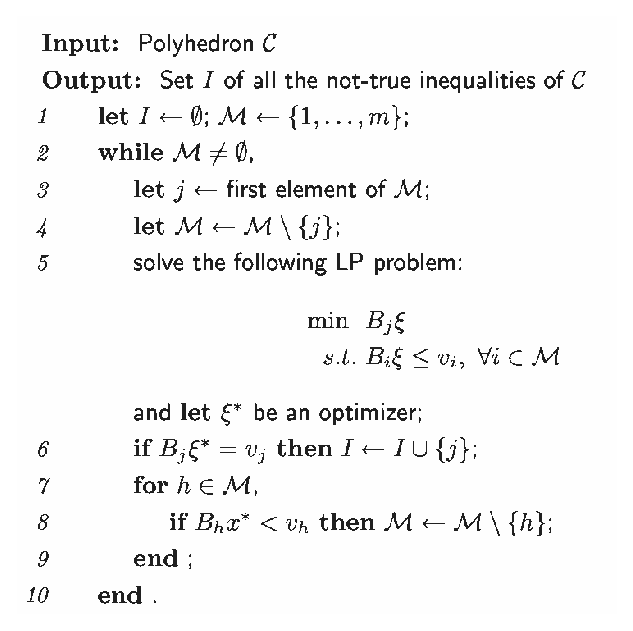
\includegraphics[width=0.6\textwidth]{algorythm1.eps}


\bigskip


\bigskip
��������� �������� ��������� ����������� ��������� ��� ����������� ����������� $n^{'} \leq n$ ����������� ��������� ��������������� $\mathcal{K}$, ����������� $K^*$, �, ����� $n^{'} \leq n$, �� ������� ���������, ������������ $\mathcal{K}$. 
\bigskip

\begin{algorithm}[H]
    \DontPrintSemicolon
    \SetAlgoLined
    \SetKwInOut{Input}{Input}\SetKwInOut{Output}{Output}
    \Input{������� $G, S, W$}
    \Output{����������� $n^{'} \leq n$ ����������� ��������� ��������������� $\mathcal{K}$, ������� �������� $k^{*}$, ���� $n^{'} \leq n$, ����� ��� $\mathcal{K} = \{ x \in \mathbb{R}^{n}  \ Tx = Z \}$}
    \BlankLine
    ����������� �������� ����������� �� ����������� \ref{alg:1}\;
    \eIf{�������� ����������� �� ��������} {
        $\mathcal{K} \leftarrow \mathbb{R}^{n}$
    }
    {
        �������� $\mathcal{P}_a \triangleq \{ (z,x) : G_{a}z - S_{a}x = W_a\}$ 
        ���� ���������� �������� ����������������, ���������� ����� ����� �� �������� ����������\;
        $\{u_1,...,u_{k^{'}}\}$ - ����� ���� $G_{a}^{'}$\;
        \uIf{$k^{'} = 0$} {
            $\Pi_{\mathbb{R}^{n}}(\mathcal{P}_a)$ � $K^*$ �������������\;
            $\mathcal{K} \leftarrow \mathbb{R}^{n}$
        }
        \Else {
            $\mathcal{K} \leftarrow \{ x\ |\ Tx = Z \}$, ��� \;
            $$
                T = - \begin{bmatrix}
                    u_{1}^{'} \\
                    \vdots \\
                    u_{k^{'}}^{'}
                  \end{bmatrix} S_a,\ Z = \begin{bmatrix}
                    u_{1}^{'} \\
                    \vdots \\
                    u_{k^{'}}^{'}
                  \end{bmatrix} W_a
            $$
        }
    }
    \caption{}
\end{algorithm}

\bigskip

� ������ ����������� ����������, � ����������, �� ����� ��������, ����� ������������, ��� ��������� $K$ ����� ����������� $n$ � $\mathbb{R}^n$.


%%%%%%%%%%%%%%%%%%%%%%%%%%%%%%%%%%%%%%%%%%%%%%%%%%%%%%%%%%%%%%%%%%%%%%%%%%%%%%%%
\subsection{����������� ����������� ��������}\label{critical-regions}
%%%%%%%%%%%%%%%%%%%%%%%%%%%%%%%%%%%%%%%%%%%%%%%%%%%%%%%%%%%%%%%%%%%%%%%%%%%%%%%%

� ���� ������� �������� ������ ��������� mp-LP, � ������ ��������� ���������� ����������� �������� $CR_{A_i}$ � �������� ������������ ��������� $K$. ����� ����� �������, ��� ��� ������ ��������� ���������������� �������� ����� � ����������� ��������������. �������� ����������� ������� ����� ����� � ������ \cite{Borelli}.

� ���� ��������������� �����, ��� ������� �������� ��������� $x\in K^*$ ������� ������������ ����������� ������� $z^0(x)$, �.�. $Z^0 (x) = \{z^0 (x)\}$,  $x\in K^*$. 

� ��������� ������������: 
\begin{itemize}
\item ������ ������������ ��� ��������� $H$-������������� ������������� ����������� ��������, 
\item ������� ����������� ����������� ��� ���������� ������� ������������ ������� $z^0 (x)$, $x\in K^*$, 
\item ������������ ������ ��� ��������� ������� ������������ �������� $J^0 (x)$, $x\in K^*$. 
\end{itemize}    
    
������������ ������ ��� (\ref{1multy}) ����� ���
\begin{equation}\label{1critical}
    \begin{split}
       & \max_y(W + Sx)'y,\\
    %    \st 
       & G'y = c,\\ 
           & y \leq 0.
    \end{split}
\end{equation}

������ � ������������ ������������ � ������� ����������� ����������� ��� ����� (\ref{1multy}), (\ref{1critical}) ����� ���
\begin{equation}\label{11critical}
    \begin{split}
            \text{������ ������������:} & \ Gz \leq W + Sx, \\
            \text{������������ ������������:} & \ G'y = c,\ y \leq 0, \\
            \text{������� ���. �����������:} & \ (G_{j}z - W_j - S_{j}x)y_i = 0, \ j \in J.
        \end{split}
    \end{equation}


������� ������������ ������ ���������� $x_0 \in \mathcal{K}$ � ����� ������ � ������������ ������ (\ref{1multy}), (\ref{1critical}) ��� $x = x_0$. ����� $z^0_0$ � $y^0_0$ --- ������� ������ � ������������ �����, ��������������. �������� $z^0_0$ ���������� ��������� ����������� ���������
\begin{equation}\label{2critical}
    \begin{split}
        A(x_0) \triangleq \{ j \in J: G_{j}z^0_0 - S_{j}x_0 - W_j = 0 \}\\
        NA(x_0) \triangleq \{ j \in J: G_{j}z^0_0 - S_{j}x_0 - W_j < 0 \}\\
    \end{split}
\end{equation}
�, �������������, ����������� ������� $CR_{A (x_0)}$.

�� ������������� ������� $y^0_0$ �����������, � �� ����������� ����������� ������� �������� $y^0_0$ �������� ����������� ��� ���� $x \in CR_{A (x_0)}$. �����, �������� ������� ��������������, ������� ������������ �������� � $CR_{A (x_0)}$ ������������ ���
\begin{equation}\label{3critical}
   J^0(x) = (W + Sx)'y^0_0, \ x\in CR_{A (x_0)},
\end{equation}
� �������� �������� �������� $x$ �� $CR_{A (x_0)}$, ��� ������� � ������� \ref{8theorem}. 

����� ����, ��� ������������ ��������� (\ref{2critical}) ������� ������ ������������ ����� ���������� � ����:
\begin{equation}\label{4critical-a}
    G_{A}z^0(x) = W_A + S_{A}x,   
    \end{equation}
\begin{equation}\label{4critical-b}
    G_{NA}z^0(x) < W_NA + S_{N A}x.
    \end{equation}
� ���������� ������������ ��������������� ������ ������� �����������, � ������� (\ref{4critical-a}) ����� ���� ������, ����� �������� ������� $z^0 (x)$. ����������, ��������� (\ref{4critical-a}) �������� ������� �� $l$ ��������, ��� � ���������� ������ ��������������� $l = s$ --- ����� �������� �����������. �� (\ref{4critical-a}) �������, ���
\begin{equation}\label{z0}
    z^0(x) = -G^{-1}_{A} S_{A} x + G_{A}^{-1}W_A = Ex + Q,
\end{equation}
������ ������� ���������� $z^0$ �� $x$. 

�� ������� ������ ������������ (\ref{4critical-b}) �������� ��������� ������������� ����������� ������� $CR_{A (x_0)}$
\begin{equation}\label{CR}
    G_{NA}(Ex + Q) < W_{NA} + S_{NA}x.
\end{equation}
�� ��������� $\overline{CR}_{A (x_0)}$ ����� ��� $G_{NA}(Ex + Q) \le W_{NA} + S_{NA}x$.

����� ����������� ����������� ������� $\overline{CR}_{A (x_0)}$ ���������� ����������� ���������� ����� ������������ $R^{\text{rest}} = K \ \backslash \ \overline{CR}_{A (x_0)}$ � ������� ����� ����������� �������.

����������� ������ � ��������� ���������� ������������ ��� ��������� � \cite{Dua57} � ��������� ������� � \cite{Bemporad25}. ����� ������������ �������, ������� ������������ ��������� ������������ ��������� ����������� ��������.
\begin{theorem}\label{9theorem}
    ����� $Y \subseteq \mathbb{R}^n$ --- ������������,  $R_0 \triangleq \{x \in Y: Ax \leq b\}$ --- ������������� ������������ $Y$, ��� $b \in R^{m \times 1},\  R_0 \not = \emptyset$. �����
    $$
    R_i =
    \left\{x \in Y:  \begin{array}{l}
        A^{i}x > b^i\\
        A^{j}x \leq b^{j},\ j < i
        \end{array}
    \right\}, \ \   i = 1,...,m, 
    $$
    ��� $b \in \mathbb{R}^{m \times 1}$ � ����� $R^{\text{rest}} \triangleq \bigcup^{m}_{i=1} R_i$.
    
    ����� \begin{itemize}
    \item[i)] $R^{\text{rest}} \cup R_0 = Y$,
    \item[ii)] $R_0 \cap R_i = \emptyset,\ R_i \cap R_j = \emptyset,\ \forall i \not = j$,
    \end{itemize}
    �.�. $\{R_0, R_1, \ldots, R_m\}$ --- ��������� $Y$.
\end{theorem}

\begin{proof}
    i) ����� ��������, ��� ����� $x \in Y$ ���� ����������� $R_0$, ���� ����������� $R_i$ ��� ���������� $i$. ���� $x \in R_0$, �� ��������� ��������. � ��������� ������, ���������� ����� ������ $i$, ��� $A^{i} x > b^i$. ����� $i^* = \min_{i \leq m} \{ i: A^{i}x > b^{i} \}$. ����� $x \in R_{i^*}$, ��������� $A^{i^{*}} x > b^{i^{*}}$ � $A^{j} x \leq b^{j},\ \forall j < i^*$, �� ����������� $i^*$.

    ii) ����� $x \in R_0.$ ����� �� ���������� �� ������ $i$ ������, ��� $A^{i} x > b^i$, �� ���� �������, ��� $x \not\in R_i,\  \forall i \leq m$. ����� $x \in R_i$ � ������� $i > j$. ��������� $x \in R_i$, �� ����������� $R_{i} (i > j)$ ����� $A^{j}x \leq b^j$, �� ���� �������, ��� $x \not \in R_j$.
\end{proof}



% %%%%%%%%%%%%%%%%%%%%%%%%%%%%%%%%%%%%%%%%%%%%%%%%%%%%%%%%%%%%%%%%%%%%%%%%%%%%%%%%
% \subsection{���������� mp-LP ���������}
% %%%%%%%%%%%%%%%%%%%%%%%%%%%%%%%%%%%%%%%%%%%%%%%%%%%%%%%%%%%%%%%%%%%%%%%%%%%%%%%%

% ����������� �� ����������� ���� ����������, ������� mp-LP ����� ���� �������� � ��������� ��������� (\ref{critical-regions}). �������� ��������, ��� �������� ���������� ��������� ������������ ��������� � ������� ������. �������� ����� ���� ������������� ��� �������� ����������� ��������, ��� ��� ���������� � (\ref{5theorem}), ������� �������� ��������� ��������, ������ �������� ��� ���������. � ���� ������ �������� ������ ����������� � ������� ��� ����������� �������, ������� �� �������� ���������������, ����� ������� ���������� ��������� ��������� ����������. � ������������ ����� ������ ����� ��������� �� �������� �����������, ��������� ������� �������� � ����������� �������� ������������ ��������� �� $x$.


%%%%%%%%%%%%%%%%%%%%%%%%%%%%%%%%%%%%%%%%%%%%%%%%%%%%%%%%%%%%%%%%%%%%%%%%%%%%%%%%
\section{Multi-Parametric Toolbox}\label{2sec:problem-formulation}
%%%%%%%%%%%%%%%%%%%%%%%%%%%%%%%%%%%%%%%%%%%%%%%%%%%%%%%%%%%%%%%%%%%%%%%%%%%%%%%%

Multi-Parametric Toolbox (��� MPT) - ��� ����� ������������ �� ������ Matlab � �������� �������� ����� ��� ��������������� �����������, �������������� ��������� � ����������� ���������� �������.
�������������� ���������� ������� ������ ����������, ���������������� � ������� � ��������� ��� ������������ �������.
���������� � ���������� ������ ������������ ���������� ����� ���� �������� � ���� ���������� � ���� ���� �� C ��� ���������� �� ������� ���������� � �������������� Real Time Workshop.

����������� ���������� ������������� �������-�������-��������� (PWA) ��������� �������� ��������
������� � ������������������ ���������� ��-�� �������� ���������� ������� �������
� �� �������. ����� Multi-Parametric Toolbox (MPT) �������� �������������� ����������� ��������������
�������� ��� ��������� ������������ �������� ����� ��� ����� ����� ������������ ����������
� ����� ���������������� Matlab. �������������������� �����������������, �������� ���
������ ������������ ����������� �������� � ���������� ������. ��������������� ������� ��������� �����
�������� ����� ����� PWA. � ���������, ������������ ��������� ����������� �� ������������ ��������� �
��� ������� �� ���� ������� ����� ������������ ���������� �������� ��� ���� �������� �������.
��� ������������ �����, ���������� �������� ����� ����� ���� ������� ��� ������������
�������� ������� � ����������� ������� ��������������������� ����������������.
� ��������� ����� ������� ���������������� ����������� ���������� � ������������ ����������� �������� (CITOC)
����������� ���������� �������-��������� ��������� ����� ������� ������� ������� � �������������.
����������, ��������� ������� PWA ������������ ����� ������ ���������� ��� ������������� ���������� ������ � ��-�� �� ��������������� ��������� ��������. ��������� ��� ����������
����������� � �������� ������ ��� ������ PWA � ������������� ���� ������������ ��� ������������� � ���������
����, � ����� �������� � ���� ��������������.
� ������� ������������ �������� �����, ������� ������������ �������� ��������� ������ �������, ����� ��������
�������� ����������� �� ������������ ������� ������� ��� ������ PWA.
�������� �� ��, ��� �������������������� ������� �������� �� ���������� ���������� ������ �������� �����,
���������� ����� ������ ����� �������������� ��� ������� �������. ��� ������� �� ������
������� ��������� �������������������� ��������, �� � �������� ��-��
����������������� ���������� ��������� ����� ���������, ������� ����� ���������, ����� ����������
����������� � ������ ������������� ����������������.


\chapter{���������� ���������������� ���������������� � ������� ������� � MPC}\label{chap2}

�� ������� ������ ������������ ���������� � ���������� ����������� �������� �����. � ����� ������� ����� �������������� �������������������� ����������������, � ����� ������� ����� ����� ��������� ������� � �������� ������ �� ���������, � ����� ��������� ���������� ��� ��� ������������ ����������.

� ����� ���������� ��������������� ���������������� �������� �������� �������, ������������ ��� �������� � ���������� ������� ������������ ���������� � �������� ������. ����������, �� ����������� �������� ������ ������������ ���������� � ���� �������������� ��������, � ������� ������� ������������������ �������� �������� �����������.
� ����������� �� ������������ ������ �������, ��������� ����������� � ������������ �������, ���������� ������ �������������� ���������.
������� ��������� ������������ ������� ������ � ������� ��������� � ����������� � �������� ���������, ������� ������ �� ������� �������������� ���������.
�� ������� ��������� ������� ��� ��������� ����� ��������� � ��������� ��������� ������� �������������������� ��������, ������������ � ��������� ������������� ��������.
��� ������������ ����� �������� ����������� ��� ���������� ������� ������������ ���������� � �������� ������.

�� ����������, ��� ������� ���� ���� ����� ������������ ���������� ����� ���� �������� � ���� �������-�������� ������ �������� �����. \\
����� ����, ����� ������������ ���������� ����������, � ������� �������� ������� � ����������.

����������� ���������� ������������� �������-�������-��������� (PWA) ��������� �������� ��������
������� � ������������������ ���������� ��-�� �������� ���������� ������� �������
� �� �������. 

\section{����� MPC}
\section{������ ����������� �������}

\chapter{��������� ������������}\label{chap2}

� ��������� ����� �������� ��� ��������� ������������� �� ����������� ���-����������� � ������ ������������ �������� ������� � ������������� �������� ����� ����� � ����������� ��� � �� ���������� ������� ����������� �������� ������ � �������� ������ ������������ ����������.

%%%%%%%%%%%%%%%%%%%%%%%%%%%%%%%%%%%%%%%%%%%%%%%%%%%%%%%%%%%%%%%%%%%%%%%%%%%%%%%%
\section{���������� ���������������� ���������������� � MPC}\label{2sec:parametric-programming-mpc}
%%%%%%%%%%%%%%%%%%%%%%%%%%%%%%%%%%%%%%%%%%%%%%%%%%%%%%%%%%%%%%%%%%%%%%%%%%%%%%%%

���������� ���������� �������� ������� ����������:
\begin{equation}\label{sys1}
     x (t + 1) = \begin{bmatrix}
            1 & 1\\
            0 & 1
        \end{bmatrix}x(t) + \begin{bmatrix}
            1\\
            0.5
        \end{bmatrix}u(t),
\end{equation}
c ������������� $-5 \le x(t) \le 5$ � $-1 \le u(t) \le 1$, $t= 0,1, \ldots$.

��� ������������ ������� (\ref{sys1}), ��������� ���������� �������, ��������, ��������� � ������ ���������, ���������� ������ ������������. ��� ������� ������ ������������ �������� ����� ����� ���, � ������� �������������� ������ --- �������-������������ � ���������� ��������������� $N = 7$, ���������� ���������� �� ���������� ����������� ����������  ���������� ����:
$$
    \sum_{k=0}^{N-1} \left[||x(k|\ t)||^2 + ||u(k|\ t)||^2\right].
$$

��� ������� ������� ������ ��������������������� ���������������� ���� ������ � �������������� ������ ������������ MPT.

������� ��� ������ ����� ���������:
\begin{verbatim}
A = [ 1, 1; 0,  1];
B = [ 1; 0.5];
\end{verbatim}

������ �������� ������ � ���������� ��������:

\begin{verbatim}
sys = ss(A,B,[],[],1);
model = LTISystem(sys);
\end{verbatim}

������� ����������� �� ���������� � ���������:

\begin{verbatim}
model.x.min = [-5; -5];
model.x.max = [5; 5];
model.y.min = [-10; -10];
model.y.max = [10; 10];
model.u.min = -1;
model.u.max = 1;
\end{verbatim}

\noindent ��������� �������� ��������
\begin{verbatim}
R = 1;
model.u.penalty = QuadFunction(R);
model.x.penalty = QuadFunction(eye(2));
\end{verbatim}

\noindent � ������������ ��������:
\begin{verbatim}
P = model.LQRPenalty;
Tset = model.LQRSet;
\end{verbatim}

�������, ����������� ������ MPC:
\begin{verbatim}
ctrl = MPCController(model,7);
\end{verbatim}

���������� ������������� ��������� ������� ����������� �������� �� ���. \ref{fig:4-1-res}. �� ���. \ref{fig:4-1-res} �) ������������ ���������� �������� ����� (����������� �����������, �������� �� ������ � ���������� ��������) ���  ���������� ��������� $x_0 = (3, 1)$. �� ���. \ref{fig:4-1-res} b) ���������� ��������� ���������� ������� �� ����������� ������� � ���������� ��������� ������� ��� ���������� ��������� ��������. �� ������� �����, ��� ������ ������������ ������� ������.

% \begin{figure}[h!]
%     \centering
%     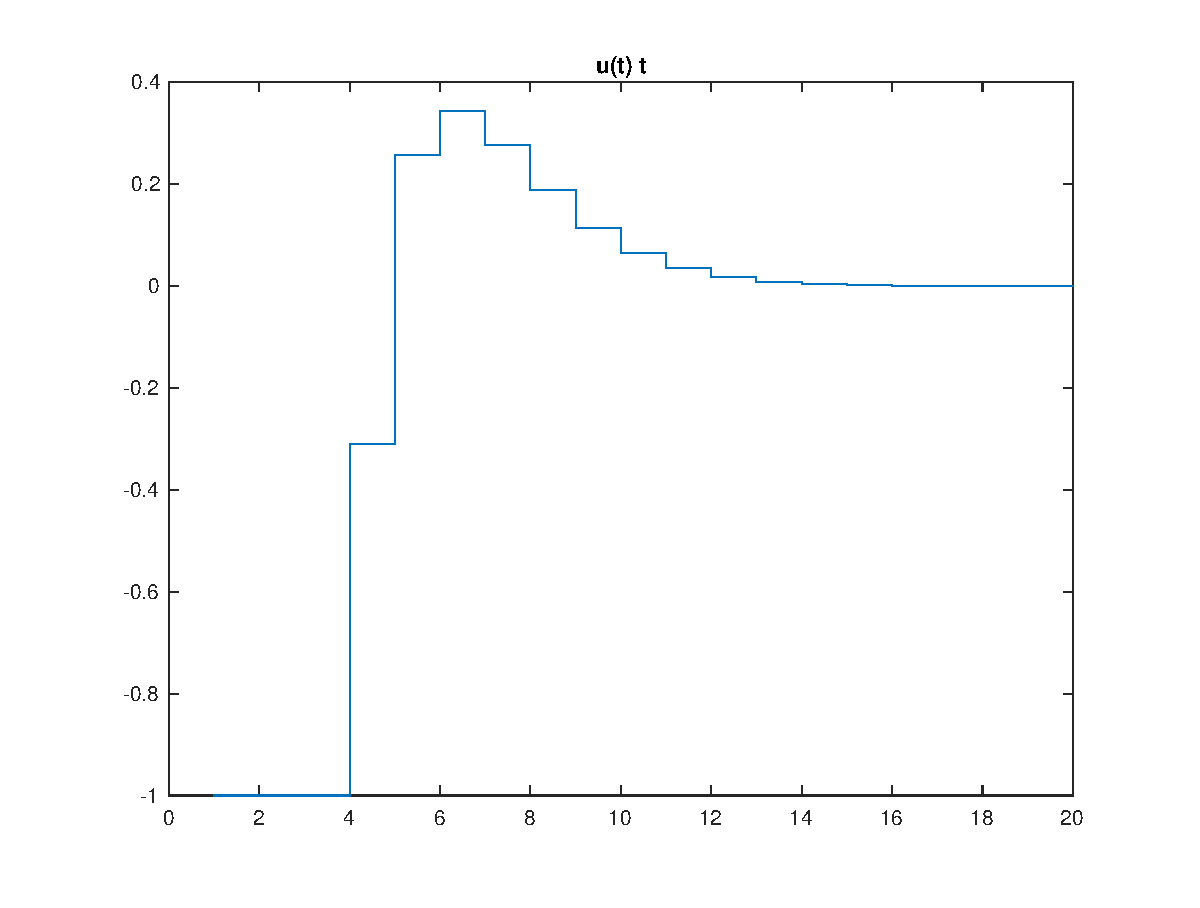
\includegraphics[width=0.6\textwidth]{u-mpc.eps}
%     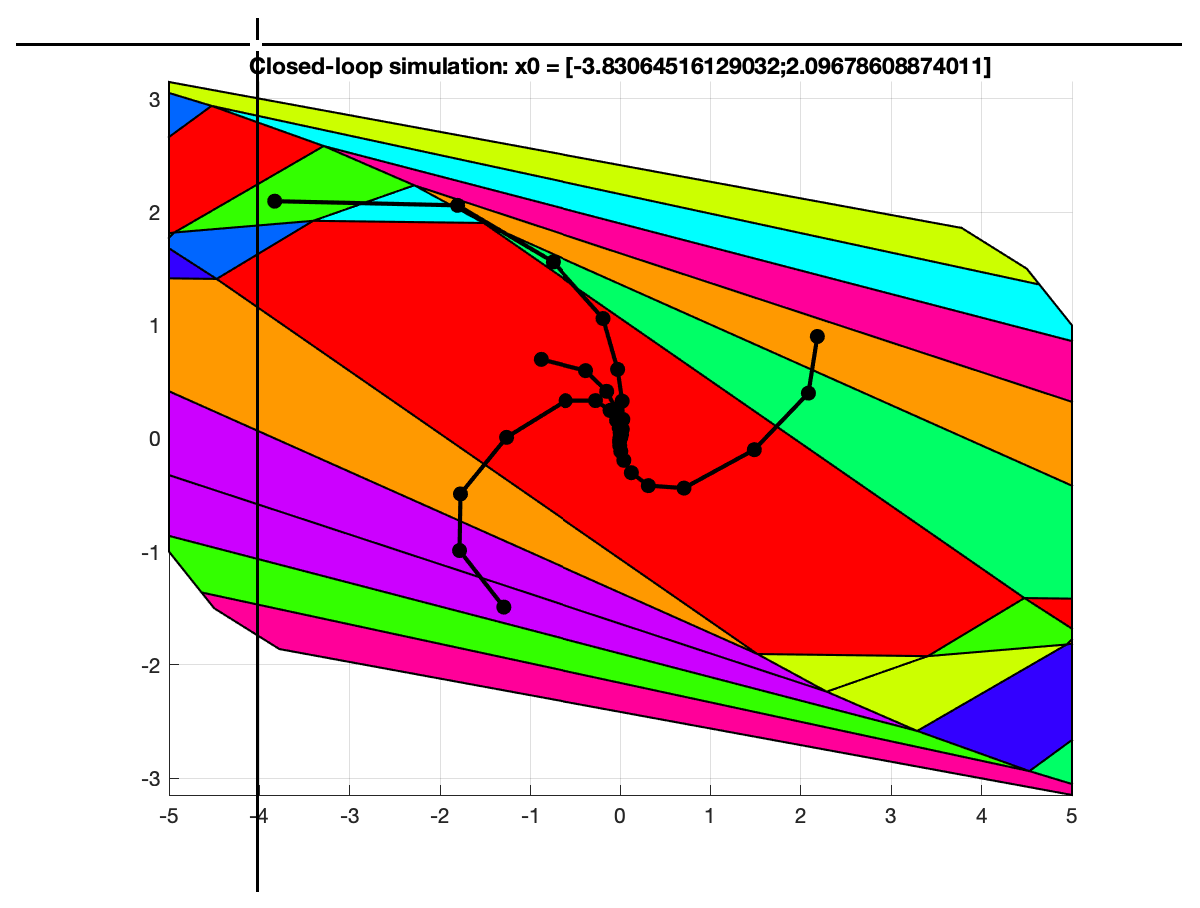
\includegraphics[width=0.6\textwidth]{controller-partition.eps}
%     \caption{����������}
%     \label{4-1-res}
% \end{figure}

\begin{figure}[h!]
    \centering
    \begin{subfigure}[b]{0.4\linewidth}
      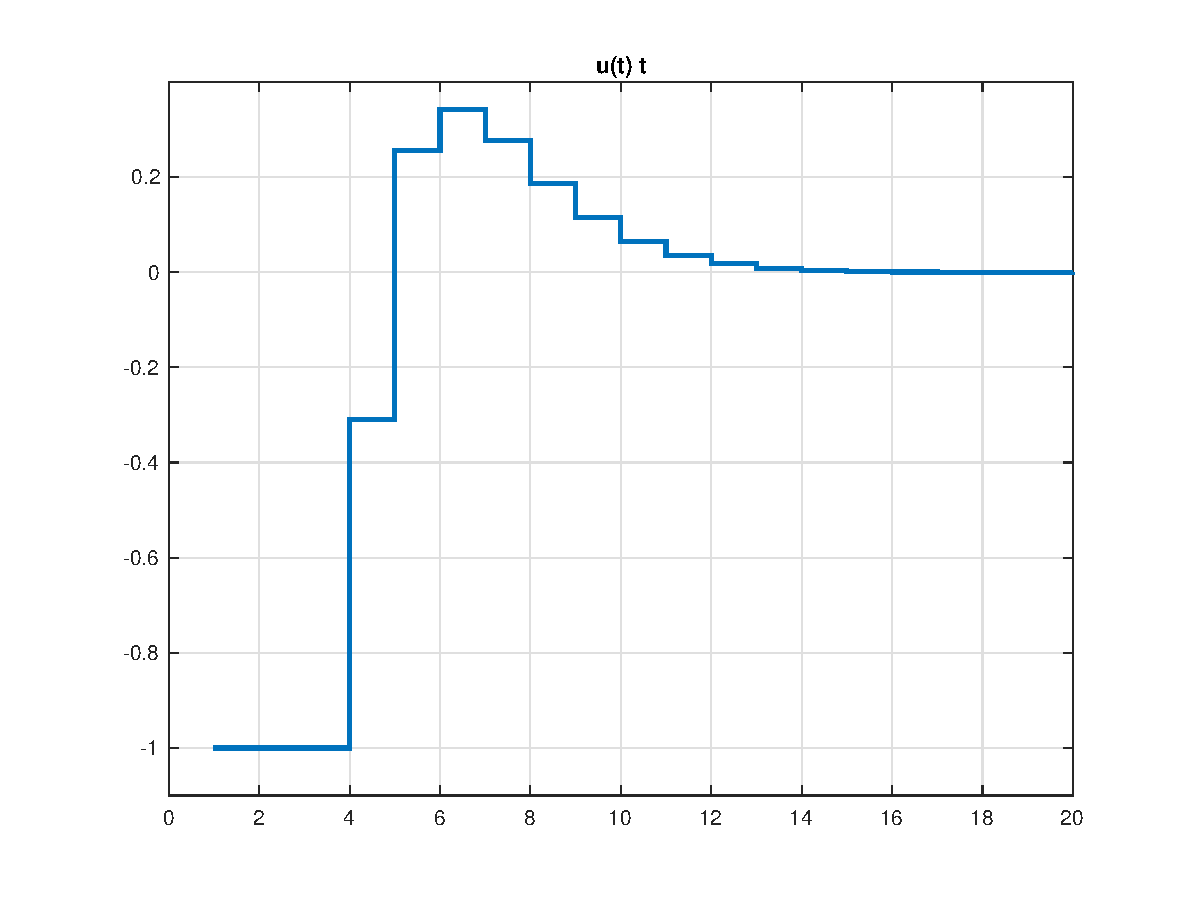
\includegraphics[width=\linewidth]{pctr-u.eps}
      \caption{����������� �����������}
    \end{subfigure}
    \begin{subfigure}[b]{0.4\linewidth}
      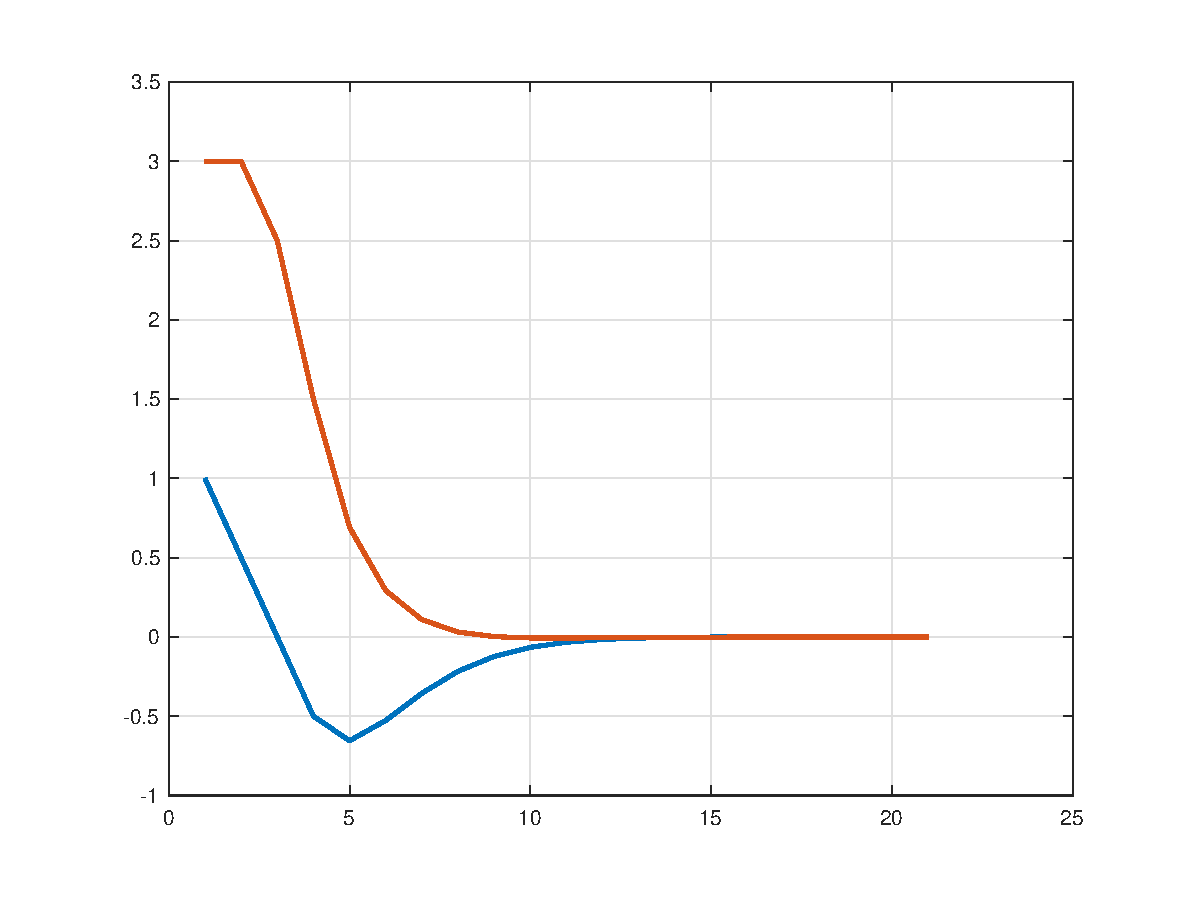
\includegraphics[width=\linewidth]{pctr-x.eps}
      \caption{���������� X}
    \end{subfigure}
    \begin{subfigure}[b]{0.4\linewidth}
      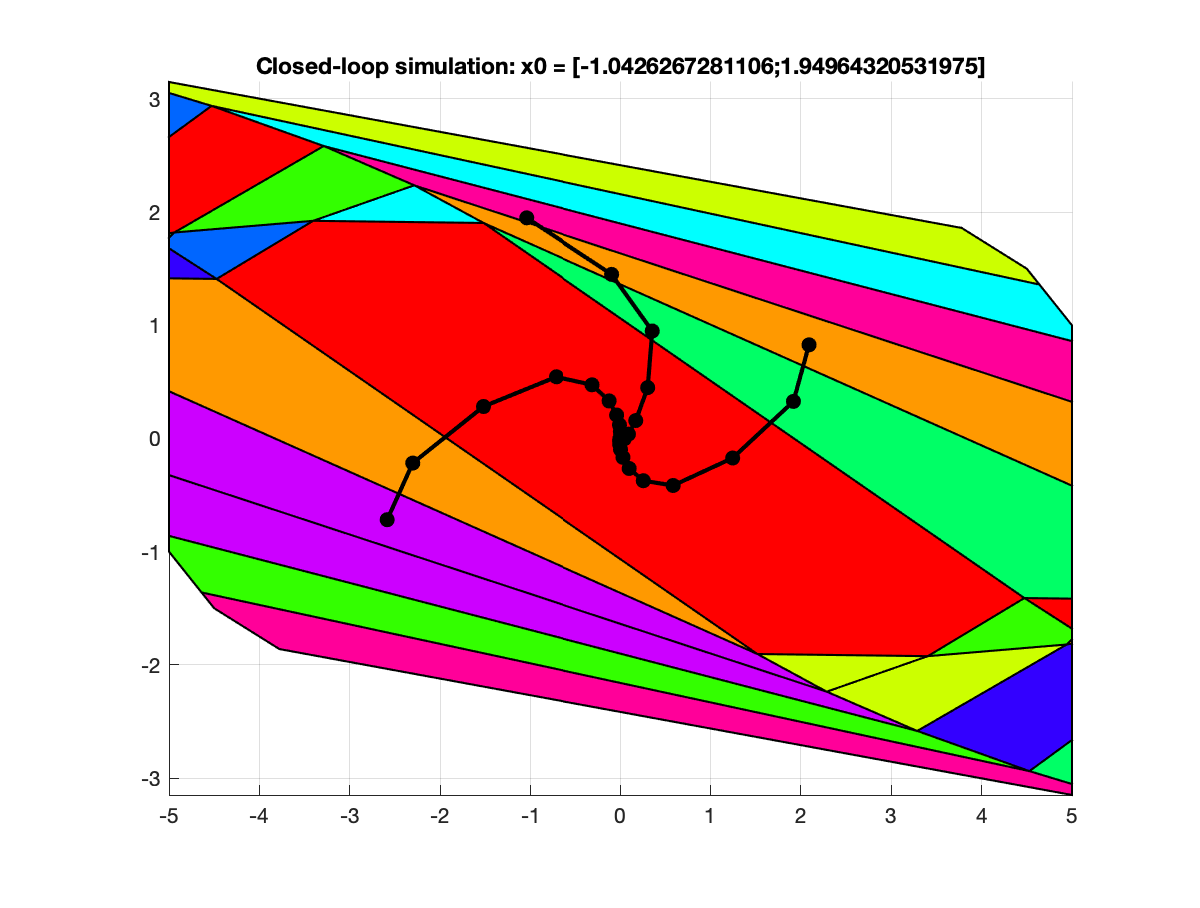
\includegraphics[width=\linewidth]{pctr-expl.eps}
      \caption{����������� ������� � ���������� ��������� �������  ��� ������ ��������� ��������}
    \end{subfigure}
    \caption{����������}
    \label{fig:4-1-res}
  \end{figure}
%%%%%%%%%%%%%%%%%%%%%%%%%%%%%%%%%%%%%%%%%%%%%%%%%%%%%%%%%%%%%%%%%%%%%%%%%%%%%%%%
\section{���������� ���������������� ���������������� � ������ ������� ����������� �������� �������}\label{2sec:parametric-programming-mpc}
%%%%%%%%%%%%%%%%%%%%%%%%%%%%%%%%%%%%%%%%%%%%%%%%%%%%%%%%%%%%%%%%%%%%%%%%%%%%%%%%

� �������� ������� ���������� ������ ����������� ������������� ������� ������� �������, ��������� �������� � ������� �������� ����������� ������� �������� ������������ �����������:
$$
    J(u) = \int_0^{t_f}|u(t)|dt \to \min,
    $$
$$
        \dot{x_1} = x_2,\\
        \dot{x_2} = -x_1 + u,
$$

� ������������� $-10 \le x \le 10$ � $-1 \le u(t) \le 1,\ t = 0,1, \cdots$. 

���������� �������� ��������: $t_0 = 0, t_f = 10$, ����� �������� ����������� ������� ������ $N=20$, ����� ������ ����������� $h=0.5$.

��� ������������� ���, ���������� �������������� ��������������� ������ ��� ������������������ �������. ��� ����� ������������� ���������� ��������� Matlab

\begin{verbatim}
sys = ss(A, B, [], []);
sysd = c2d(sys,tf/N,'zoh');
\end{verbatim}

� ���������� ����� �������� ��������� �������

$$
    A_d = \begin{bmatrix}
        0.8776 & 0.4794\\
        -0.4794 &  0.8776\\
    \end{bmatrix}
    B_d = \begin{bmatrix}
        0.1224 \\
        0.4794 \\
    \end{bmatrix}
    $$
����������� ���������� ������� $x(t+1)  = A_d x(t) + B_d u(t)$, $x(0)=0$, $t=0, 1, 2, \ldots$.


� ���  ����� ������ ��� ��������� ������, ����� �������� �� � $mpt constructMatrices$, �������  ������������ ����� �������, �� ���� ������� �������� ��������� $probStruc$t � $sysStruct$.
��������� ������� $sysStruct$ ����� �������� �� ������ $A$, $B$, $C=(0, 0)$, $D=0$, ����������� �� $x$ ($x_min$ � $x_max$) � ����������� �� $u$ ($u_min$ � $u_max$). ��������� ������ $probStruct$ � ���� ������� ����� �������� �� ��������� �����, ����� $N$, � ����� $Q$, $P_N$, $R$ � ��. � ��������������� ������ ��� �������� �����, ��� $Q = 0$, $P_N = 0$, $R=1$, ����� �����������.


����� ���������� ������ ��������� ������ � Matlab �������� ���, ��� �������� ����:

\begin{verbatim}
sysStruct.A= Ad;
sysStruct.B= Bd;
sysStruct.C= [0 0];
sysStruct.D= 0;
\end{verbatim}

\begin{verbatim}
sysStruct.xmin = [-10; -10];
sysStruct.xmax = [10; 10];
\end{verbatim}

\begin{verbatim}
sysStruct.umin = -1;
sysStruct.umax = 1;
\end{verbatim}

\begin{verbatim}
nx = size(A, 2);
probStruct.norm=inf;
probStruct.Q=[0 0; 0 0];
probStruct.P_N=[0 0; 0 0];
probStruct.R=1;
probStruct.N=N;
probStruct.subopt_lev=0;
H = [eye(nx); -eye(nx)];
K = eps*ones(nx*2,1);
probStruct.Tconstraint=2;
probStruct.Tset = polytope(H, K);
\end{verbatim}

����� ���������� ������ ����  ����� ����� ��� ��������� ��������������� ������, ��������������� � ���������, ������� ����� ������, ��������� ��������� ���������. 

����� ����� �� ��������� $mpt constructMatrices$ ���������� ����� $Opt$, ������� ������������� ���������� � ������� ��� ����� LP/QP/pLP/pQP/LCP/pLCP.
��� ����������� ������� ������� �������� $u$ �� ��������� ��������� $x_\tau$ � �������� �� �������. ��������� ����������� � ������ ������  �� $T_h$.

����� ������������� ��������� ���� �������� � ����� �� ������ ���� � �� �������� ���� ������� ���������� $w$.
\begin{verbatim}
for tau = 0:NN-1
    probStruct.N=N;
    Matrices = mpt_constructMatrices(sysStruct,probStruct);
    plp = Opt(Matrices);
    solution = plp.solve();
    u = solution.xopt.feval(xtau, 'primal');
    if N > NN/2
        xtau = Ad * xtau + Bd * u(1) + w;
    else
        xtau = Ad * xtau + Bd * u(1);
    end

    figure;
    solution.xopt.fplot('obj');
    xlabel('x0');
    ylabel('J(x0)');
    N = N-1;
    X = [X xtau];
    U = [U u(1)];
end
\end{verbatim}
\bigskip


�� ���. \ref{4-img-1}) ��������� ���������� ������ ��� --- ����������� ������� ��� �������� $\tau = 0$, $\tau = 2.5$, $\tau = 5$, $\tau = 9.5$.

\begin{figure}[h!]
    \centering
    \begin{subfigure}[b]{0.48\linewidth}
    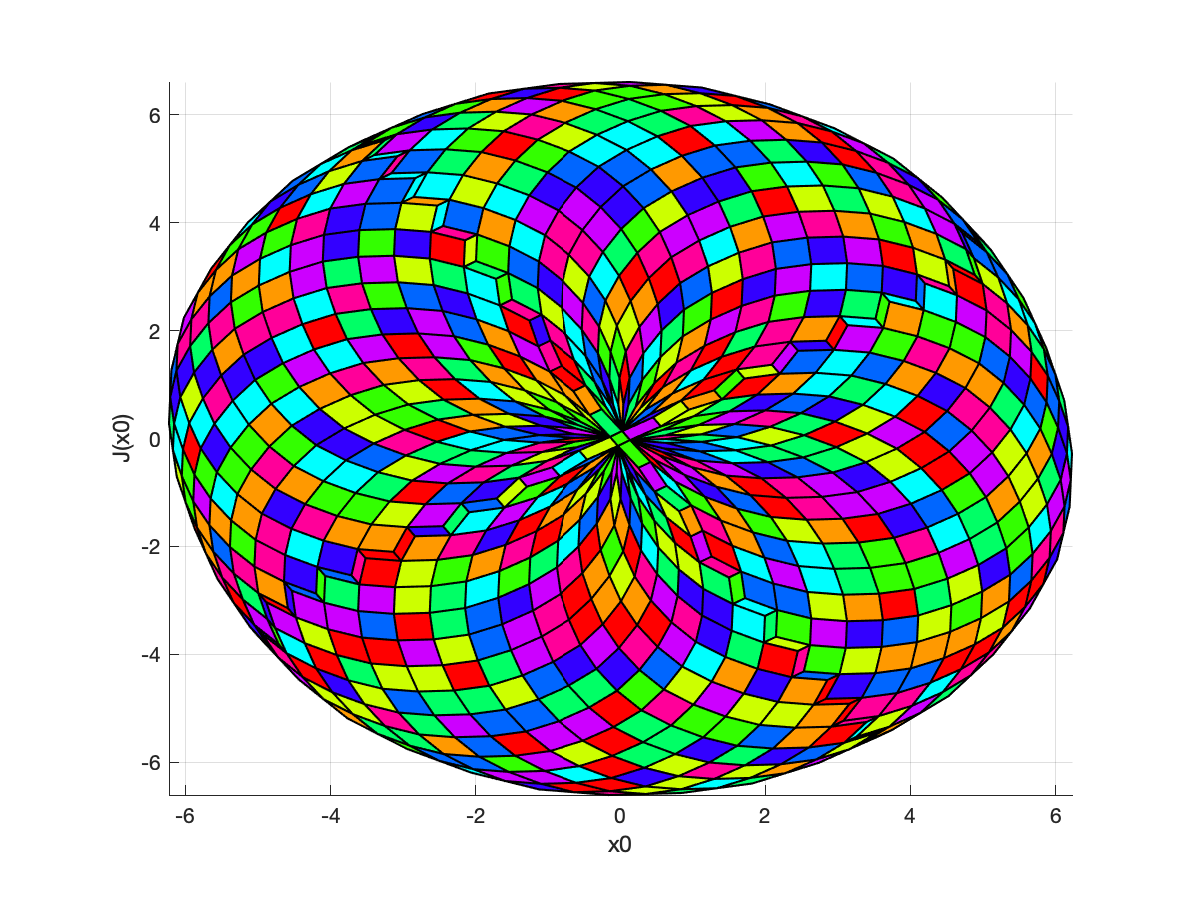
\includegraphics[width=1\textwidth]{figure1.eps}
      \caption{N = 20, $\tau = 0$}
    \end{subfigure}
    \begin{subfigure}[b]{0.48\linewidth}
        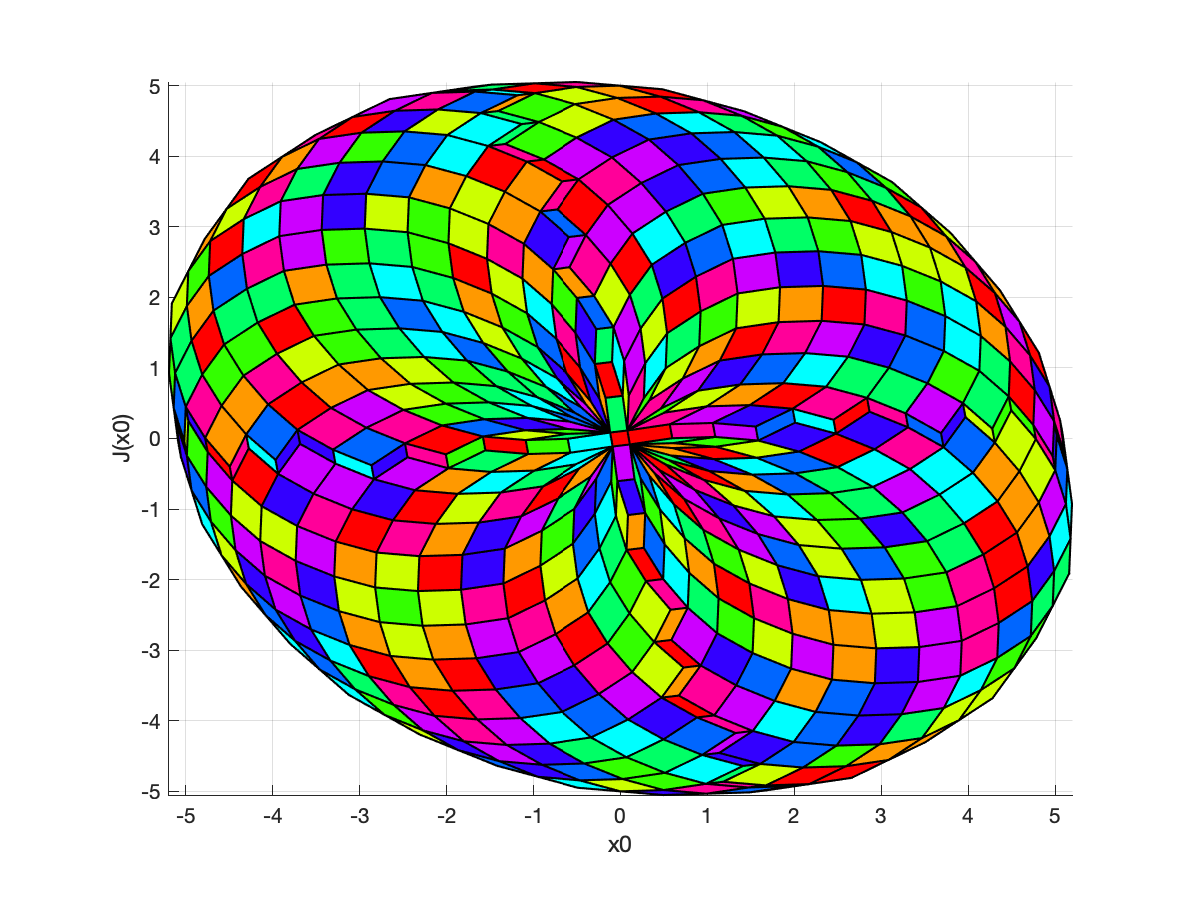
\includegraphics[width=1\textwidth]{figure5.eps}
      \caption{N = 15, $\tau = 2.5$}
    \end{subfigure}
    \begin{subfigure}[b]{0.48\linewidth}
    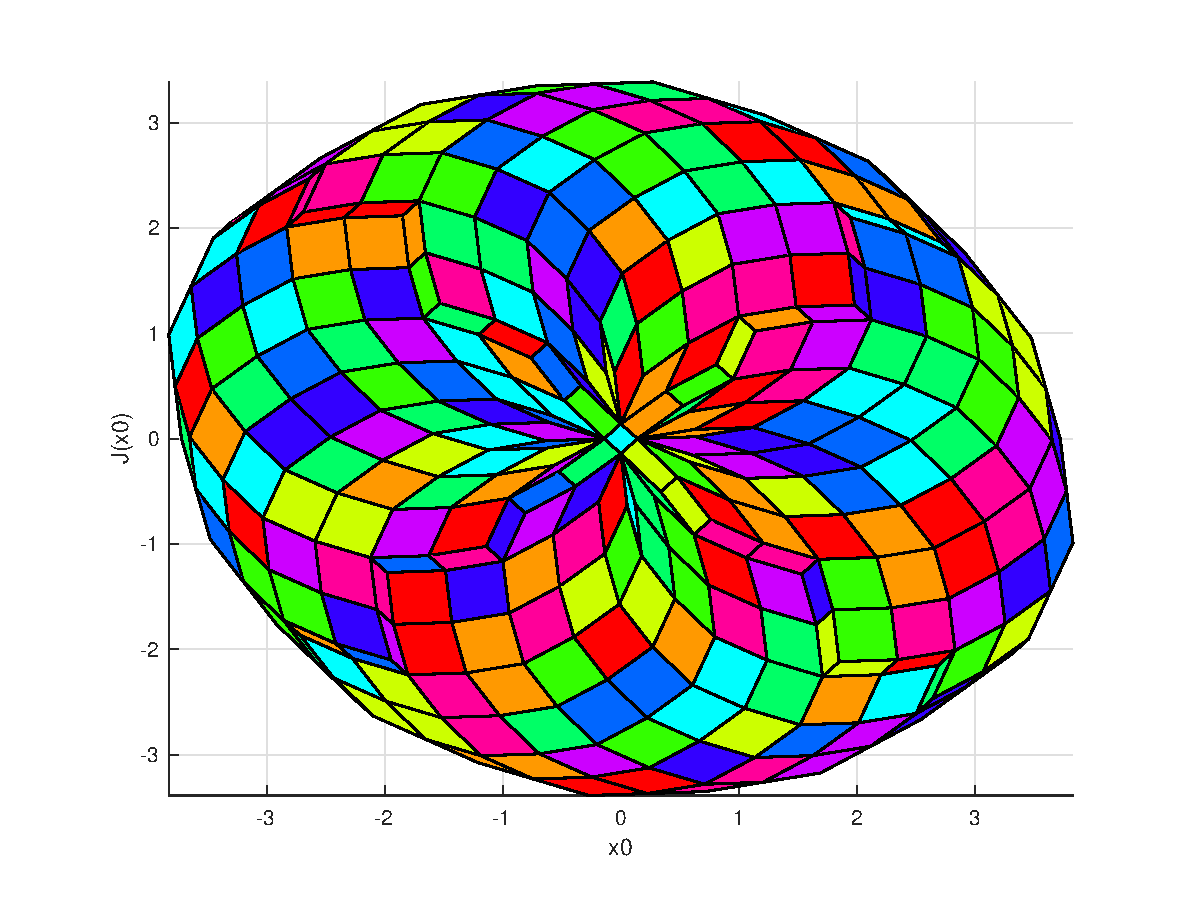
\includegraphics[width=1\textwidth]{figure10.eps}
      \caption{N = 10, $\tau = 5$}
    \end{subfigure}
    \begin{subfigure}[b]{0.48\linewidth}
        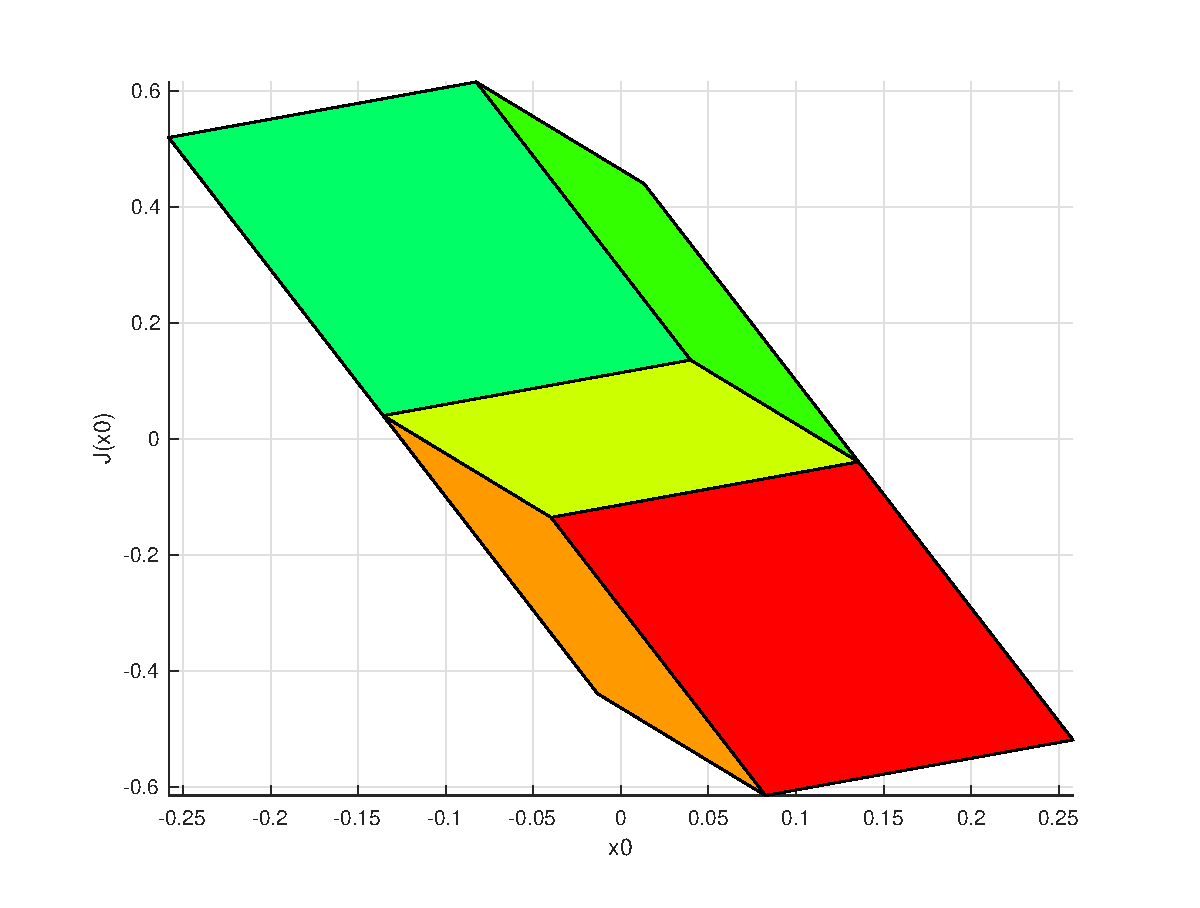
\includegraphics[width=1\textwidth]{figure20.eps}
      \caption{N = 1, $\tau = 9.5$}
    \end{subfigure}
    \begin{subfigure}[b]{0.48\linewidth}
        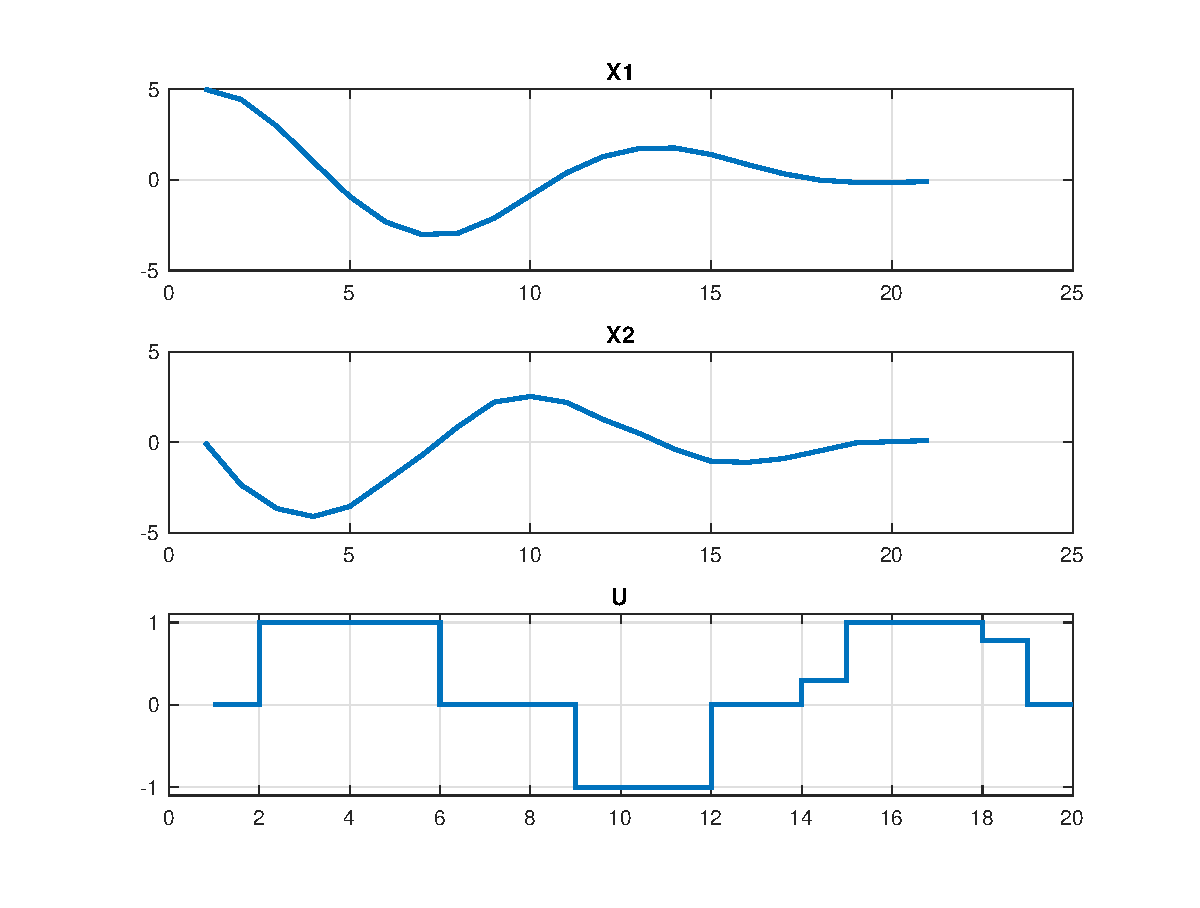
\includegraphics[width=1\textwidth]{graphics-42.eps}
      \caption{X � U}
    \end{subfigure}
    \begin{subfigure}[b]{0.48\linewidth}
        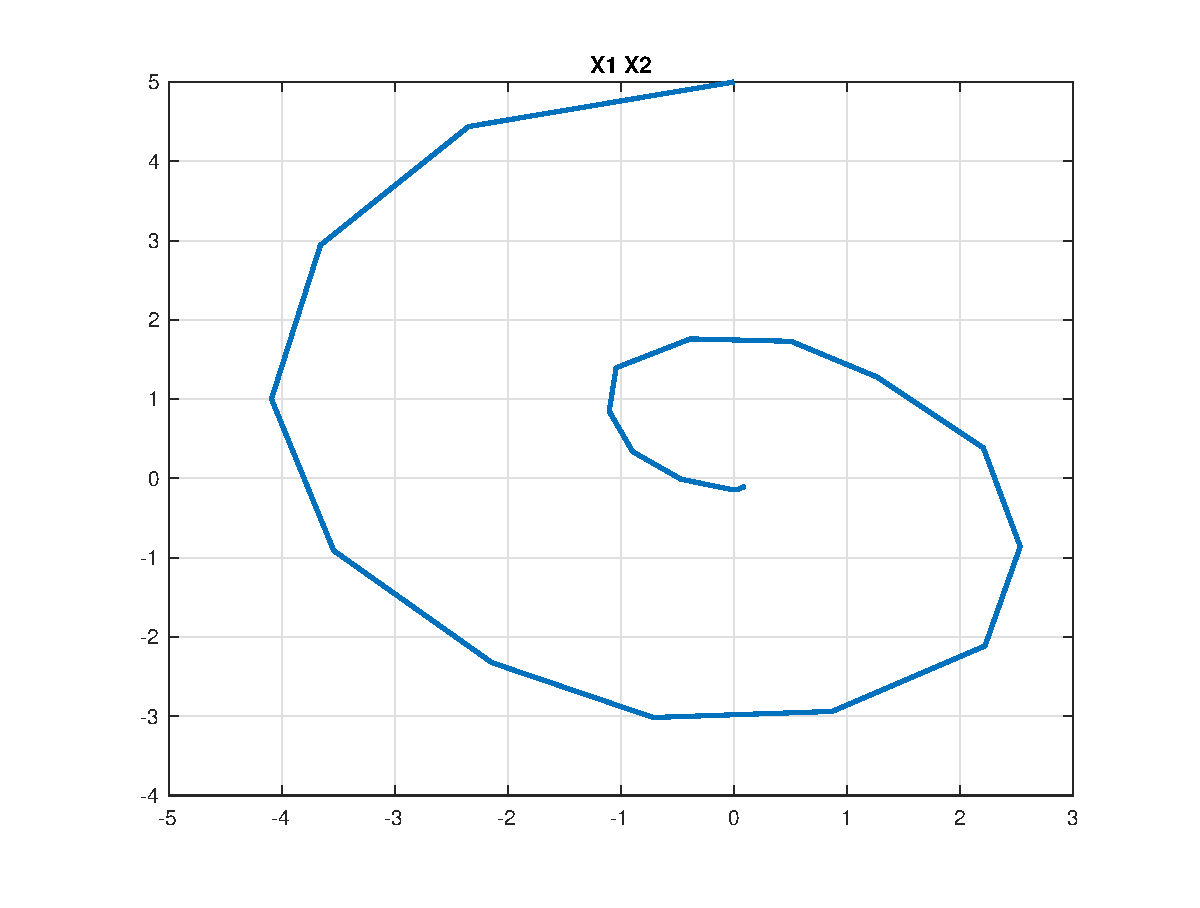
\includegraphics[width=1\textwidth]{x1x2.eps}
      \caption{$X_1, \ X_2$}
    \end{subfigure}
    \caption{����������}
    \label{4-img-1}
\end{figure}
\clearpage


\bigskip
!!!!!!!!!!!!!!!!!!!!!!!!!!!!!!!!!!

��� ���������� �� ����, ���� ������ �� �� ������ ��� ���������. ��� ��� ������ � ������� ���, � �� � �� �������, � ���� ����� ������.


!!!!!!!!!!!!!!!!!!!!!!!!!!!!!!!!!!
\bigskip

\bigskip



����� ���� ����������� ������������� ���� �� ���������� ������������ ����������� �������� �����. � ������ ����� �������������, ��� ��������������� ���������������� ����������� � ������� ������� ����������� �������� �������.

���������� ��������� ������:
\begin{equation}
    \begin{aligned}
    & x_1(t_f) \to \min,\\
    & x_2(t_f) = 0,\\
\end{aligned}
\end{equation}
�� ����������� ������� ������� �������
$$
    \begin{cases}
        \dot{x_1} = x_2,\\
        \dot{x_2} = -x_1 + u,
    \end{cases}
    x_1(t_0) = x_{10},\
    x_2(t_0) = x_{20},
$$
� ������������� $-L \le u \le L, \ t \in T = [t_0,\ t_f]$
\\
������� A ����� ���:
$$
A = \begin{bmatrix}
    0 & 1\\
    -1 & 0
\end{bmatrix}
$$
������� $b$ �������� ��������� �������:
$$
b = \begin{bmatrix}
    0 \\
    1
\end{bmatrix}
$$
������� $H$:
$$
H = \begin{bmatrix}
    0 \\
    1
\end{bmatrix}
$$

���������� ������ �������� ��������: $t_0 = 0,\ t_f = 10$.
����� ������������ ���������� ����������� ����������� � ����� $h = \frac{t_f - t_0}{100}$.
��������� ��������� � ��������� ������� ����� �������:

$c_h, d_h$ �� ������ ���� � matlab ����������� ���������� integral � Matlab, ������� ������������� � ����� ��� ������� ����:

\begin{verbatim}
for i = 1:N
    ch(i) = integral(C,t0+h*(i-1),t0+h*i,'ArrayValued',true);
    dh(i) = integral(d,t0+h*(i-1),t0+h*i,'ArrayValued',true);
end
\end{verbatim}

$u_0$, � ���� �������, ����������� � ������� ��������� linprog:
\begin{verbatim}
u0 = linprog(-ch',[],[],dh,g0,-L*ones(N,1),L*ones(N,1))
\end{verbatim}

����� ���������� $x$:
\begin{verbatim}
x = zeros(2,N+1);
x(:,1) = x0;
for i = 1:N
    x(:,i+1) = F(h)*x(:,i)+integral(@(t)u0(i)*F(t0+(i+1)*h-t)*b,t0+i*h,t0+(i+1)*h,'ArrayValued',true);
end
x1 = zeros(2,N+1);
x1(:,1) = x0;
for i = 1:N
    x1(:,i+1) = F(h)*x1(:,i)+integral(@(t)u0(i)*F(t0+(i+1)*h-t)*b+w(t),t0+i*h,t0+(i+1)*h,'ArrayValued',true);
end
\end{verbatim}


����� �� ������������ ���������� ������� ������� ���������� $w$ � ������ � ������ � ������� ��������� ��� ��� ��������:
\begin{verbatim}
    for j = 1:N
        j
        if j>90
            w = @(t)0*cos(3*t);
        end
        tau = t0 + (j-1)*h;
        g0 = g-H*F(tf-tau)*x2(:,j);
        u1 = linprog(-ch(j:N),[],[],dh(j:N),g0,-L*ones(N-j+1,1),L*ones(N-j+1,1))
        u2(j) = u1(1);

        x2(:,j+1) = F(h)*x2(:,j)+integral(@(t)u2(j)*F(t0+(j+1)*h-t)*b+w(t),t0+j*h,t0+(j+1)*h,'ArrayValued',true);
        x(:,j+1)
        x2(:,j+1)
    end
\end{verbatim}

���������� ��� ���������� �������� $x_0 = [1; -1]$ �������� �� ������� \ref{picture-primer}


\begin{figure}[h!]
    \centering
    \begin{subfigure}[b]{0.4\linewidth}
      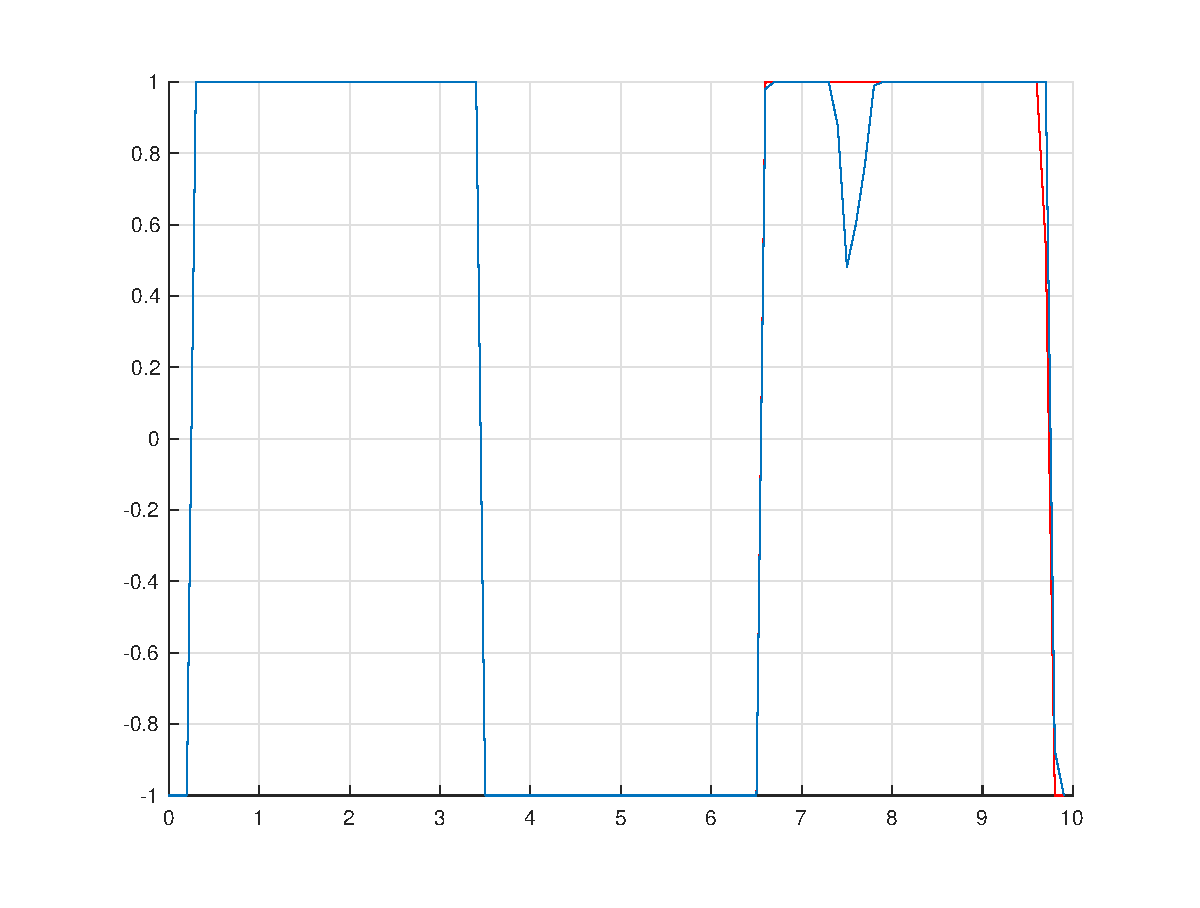
\includegraphics[width=\linewidth]{primer2-1.eps}
      \caption{X}
    \end{subfigure}
    \begin{subfigure}[b]{0.4\linewidth}
      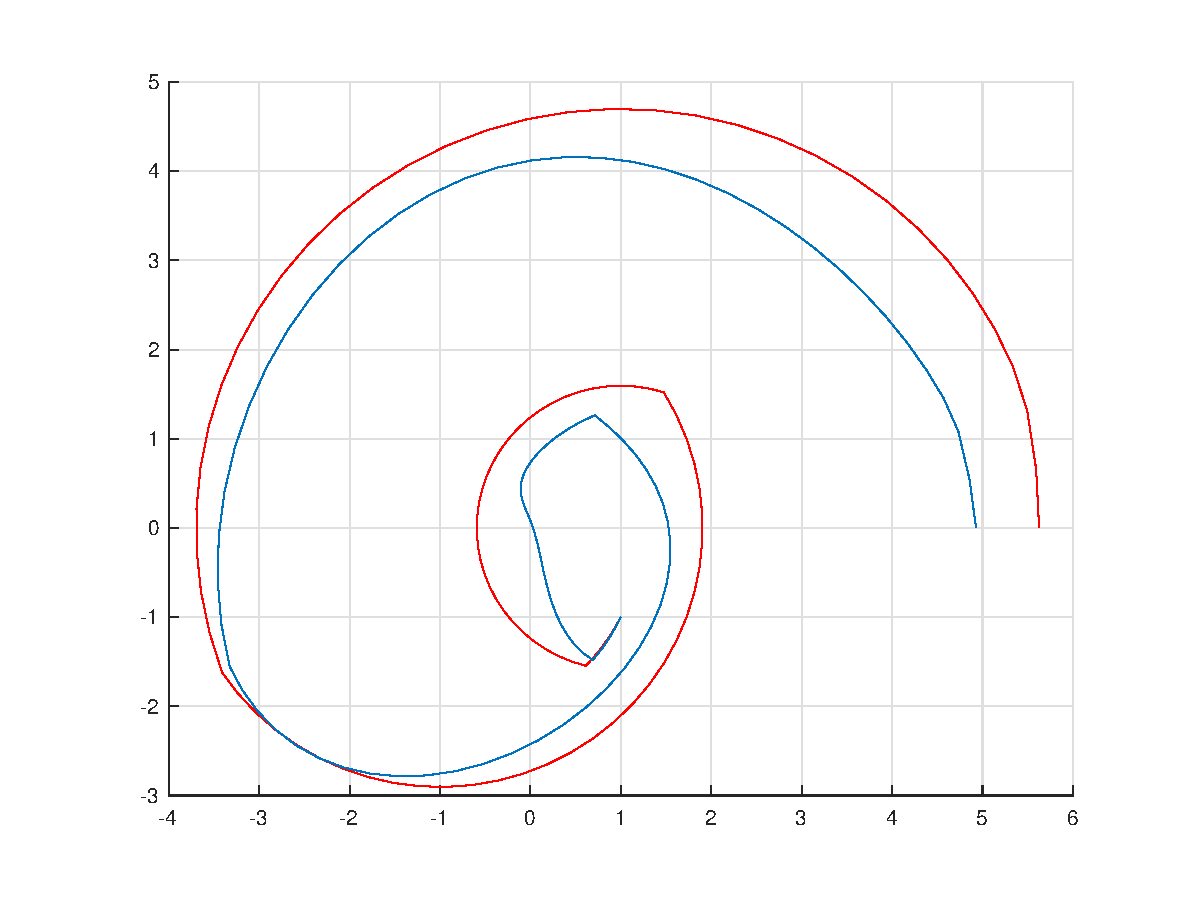
\includegraphics[width=\linewidth]{primer2-3.eps}
      \caption{U}
    \end{subfigure}
    \caption{����������}
    \label{picture-primer}
  \end{figure} 

% ************************************************************************
%   ЗАКЛЮЧЕНИЕ
% ************************************************************************

\chapter*{����������}
\addcontentsline{toc}{chapter}{����������}


� ��������� ������� ����������� ������ ������� ����������� ������� ������� �������. ��� ����������� ������ ���������� ���� �������, ���������� � ���� �������������� MPT ��� Matlab. �������� ������ ������� ���������������� ����������������. ���������� ����������������� �� ��������, �������������� ����. ����� � ������ ���� ������� �������� ���������� ������ ������������ ���������� � ������ � ���������� ���������� ����������� �������� ������.

����� ���������� ������ ������� ����������� �������� ������ � �������� ������ ������������ ���������� �� ������ ���� ���������������� ����������������, �� �������� � ���������, ��������������� � ����� ������ ���������� �� �������������� ������.

� ������ ������������ ���������� ���������� �� �������������� ������, ����� ����� MPC �� ������ ���������������� ��������� ���������������� � ����������� ���� ������� �� ���������� ��������. � ���� ������ ����������� ��������� �����������, ���������� ����� ������������� MPT ��� Matlab, � ������������, ����������� ����� ����������� �������, ��������� ��������� linprog ��� Matlab.
 



% ************************************************************************
%   СПИСОК ИСПОЛЬЗОВАННОЙ ЛИТЕРАТУРЫ
% ************************************************************************

\begin{biblio}
    \bibitem{Bellman}
    R. Bellman. The Dawn of Dynamic Programming. Dover Publications, reprint edition, 2003

    \bibitem{Pontryagin}
    Hazewinkel, Michiel. Pontryagin maximum principle. Encyclopedia of Mathematics, Springer Science+Business Media B.V. / Kluwer Academic Publishers, 2001.

    \bibitem{Hogan}
    W. M. Hogan. Point-to-set maps in mathematical programming. SIAM Review, 15(3):591�603, July 1973.
    
    \bibitem{GalNedoma}
    T. Gal and J. Nedoma. Multiparametric linear programming. Management Science, 18:406�442, 1972.

    \bibitem{Bemporad25}
    A. Bemporad, M. Morari, V. Dua, and E.N. Pistikopoulos. The explicit linear quadratic regulator for constrained systems. Automatica, 38(1):3�20, 2002.

    \bibitem{GassSaaty}
    T. Gal. Postoptimal Analyses, Parametric Programming, and Related Topics. de Gruyter, Berlin, 2nd edition, 1995.
    
    \bibitem{Berkelaar28}
    A.B. Berkelaar, K. Roos, and T. Terlaky. The optimal set and optimal partition approach to linear and quadratic programming. In T. Gal and H.J. Greenberg, editors, Advances in Sensitivity Analysis and Parametric Programming, volume 6 of International Series in Operations Research and Management Science, chapter 6. Kluwer Academic Publishers, 1997.
    
    \bibitem{Adler2}
    I. Adler and R.D.C. Monteiro. A geometric view of parametric linear programming. Algorithmica, 8(2):161�176, 1992.
    
    \bibitem{Filippi}
    C. Filippi. On the geometry of optimal partition sets in multiparametric linear programming. Technical Report 12, Department of Pure and Applied Mathematics, University of Padova, Italy, June 1997.
    
    \bibitem{Dua57}
    V. Dua and E.N. Pistikopoulos. An algorithm for the solution of multiparametric mixed integer linear programming problems. Annals of Operations Research, to appear.
    
    \bibitem{Bemporad}
    A. Bemporad, M. Morari, V. Dua, and E.N. Pistikopoulos. The explicit linear quadratic regulator for constrained systems. Automatica, 38(1):3�20, 2002.
    
    \bibitem{ChenAllgower}
    H. Chen, F. Allgower. A Quasi-Infinite Horizon Nonlinear Model Predictive Control Scheme with Guaranteed Stability. Automatica, 1998

    \bibitem{Borelli}
    Borelli, F. Constrained Optimal Control of Linear and Hybrid Systems / F. Borelli // Lecture Notes in Control and Information Sciences. - Springer, 2003. - Vol. 290. - 293 p.
\end{biblio} 

\label{lastpage}


\end{document}
